%% 第四章 检测模型改进与消融实验
\chapter{检测模型改进与消融实验}

本章介绍面向无人机小目标的检测模型改进。首先说明基础模型的选择依据，分析标准 YOLOv8n 在小目标上的结构性局限；然后详细阐述 P2 检测头与 EMA 注意力的设计、插入位置与计算开销；接着给出训练配置与消融实验结果，并从特征分辨率、注意力响应与参数效率三个角度解释结果；最后讨论模型的有效工作范围与失效模式。

\section{基础模型选型}

\subsection{规模选择}

YOLOv8 提供 n、s、m、l、x 五种规模，参数量从约 3\,M 到约 68\,M。选择何种规模需要综合考虑精度、速度与部署条件。本文的目标平台是一台配备 RTX 4060 笔记本 GPU 的普通计算机，系统需要在处理 720p 视频的同时完成界面渲染、地图更新与数据记录，因此检测模型不能占用过多显存与算力。

表~\ref{tab:model_scale} 给出了各规模在 COCO 上的参考指标（Ultralytics 官方数据）与本文实测的推理速度。

\begin{table}[htbp]
\centering
\caption{YOLOv8 各规模模型对比}
\label{tab:model_scale}
\small
\begin{tabular}{lccccc}
\toprule
\textbf{模型} & \textbf{参数量(M)} & \textbf{COCO mAP50-95} & \textbf{640 推理(ms)} & \textbf{显存(MB)} & \textbf{适用场景} \\
\midrule
YOLOv8n & 3.2 & 37.3 & 6.2 & 约 420 & 边缘/桌面实时 \\
YOLOv8s & 11.2 & 44.9 & 11.5 & 约 680 & 桌面实时 \\
YOLOv8m & 25.9 & 50.2 & 25.8 & 约 1100 & 服务器 \\
YOLOv8l & 43.7 & 52.9 & 44.6 & 约 1600 & 服务器 \\
YOLOv8x & 68.2 & 53.9 & 68.3 & 约 2200 & 离线分析 \\
\bottomrule
\end{tabular}
\end{table}

本文选择 nano 版本，原因有三。第一，在 640 输入下推理耗时约 6\,ms，端到端（含预处理、后处理与绘制）可稳定在 30\,fps 以上，满足实时监视需求。第二，参数量小，模型文件约 6\,MB，便于随桌面应用分发，也便于在 CPU 上降级运行。第三，nano 版本的容量有限，小目标能力较弱，改进空间大，能够更清晰地体现 P2 与 EMA 的作用；若直接使用 large 模型，改进带来的相对提升可能被强大的基线能力掩盖。

\subsection{标准结构的局限}

YOLOv8n 的检测头接在 P3、P4、P5 三层，对应 stride 8、16、32。对于 640$\times$640 输入，三层特征图尺寸分别为 80$\times$80、40$\times$40、20$\times$20。一个宽度为 20\,px 的目标在 P3 上仅占 2.5 个网格，在 P4 上占 1.25 个，在 P5 上不足 1 个。由于每个网格只能预测有限数量的目标，且特征在经过多次下采样后已经丢失了大量边缘与纹理信息，微小目标在标准结构上的响应非常弱。

更具体地说，小目标的检测依赖于浅层特征，但浅层特征的语义判别力不足，容易将树叶、窗户、云朵误判为目标；深层特征语义强，但空间分辨率低，小目标已经"消失"。这一矛盾是 FPN 试图解决的核心问题，但当目标小于 32\,px 时，即使 P3 层也难以提供足够的分辨率。因此，增加更浅的检测层是直接且有效的思路。

\section{P2 小目标检测头}

\subsection{结构设计}

本文在标准 YOLOv8n 的颈部增加一条自底向上的分支，将 stride=4 的浅层特征 $C_2$ 与 P3 上采样后的特征融合，得到 P2 特征图，并在其上接一个额外的检测头。设输入为 640$\times$640，各层特征图尺寸如表~\ref{tab:p2_shapes} 所示。

\begin{table}[htbp]
\centering
\caption{各检测层特征图尺寸与网格占用（640$\times$640 输入）}
\label{tab:p2_shapes}
\small
\begin{tabular}{lccccc}
\toprule
\textbf{检测层} & \textbf{stride} & \textbf{特征图} & \textbf{20\,px 目标占用网格} & \textbf{40\,px 目标占用网格} & \textbf{感受野} \\
\midrule
P2（本文新增） & 4 & 160$\times$160 & 5.0 & 10.0 & 较小 \\
P3 & 8 & 80$\times$80 & 2.5 & 5.0 & 中 \\
P4 & 16 & 40$\times$40 & 1.25 & 2.5 & 较大 \\
P5 & 32 & 20$\times$20 & $<1$ & 1.25 & 大 \\
\bottomrule
\end{tabular}
\end{table}

融合路径可以写为

\begin{equation}
P_2 = \mathrm{Conv}_{3\times3}\left(\mathrm{Conv}_{1\times1}(C_2)\oplus
\mathrm{Upsample}_{2\times}\left(\mathrm{Conv}_{1\times1}(P_3)\right)\right),
\label{eq:p2_fusion}
\end{equation}

其中 $\oplus$ 为逐元素相加。与自顶向下的 FPN 路径相比，这条"浅层直连"路径的最大特点是\textbf{传播距离短}：$C_2$ 只经过一次 $1\times1$ 卷积与一次 $3\times3$ 卷积便到达检测头，梯度回传路径也相应缩短，有利于浅层特征的训练。

\subsection{检测头配置}

新增的 P2 检测头与原有检测头结构一致，包含分类分支与回归分支，输出通道数为 $4\times16+1$（DFL 的 16 个分布参数、4 个边框参数与 1 个类别）。由于 P2 特征图尺寸是 P3 的 4 倍，检测头的计算量与显存占用显著增加。本文通过在 P2 分支使用较少的通道数（64）来控制开销。

\subsection{计算量与参数分析}

引入 P2 后，模型参数量从 3.01\,M 降至 2.93\,M，这一反直觉的现象需要解释。参数量减少的原因是：YOLOv8 的解耦头在不同尺度上共享部分结构，新增 P2 头的同时，颈部的一部分高层卷积被替换为更浅的融合路径，整体参数量略有下降。但计算量并未下降：P2 特征图的分辨率是 P3 的 4 倍，检测头在该层上的卷积计算量约为原来的 4 倍，因此 FPS 从 123 降至 90。

这一权衡是合理的：反无人机场景对召回率的要求高于对帧率的要求，90\,fps 仍远高于 30\,fps 的视频帧率，留有充足余量。

\subsection{正负样本分配}

YOLOv8 使用 TaskAlignedAssigner 进行正负样本分配，其匹配分数为分类分数与 IoU 的加权乘积：

\begin{equation}
t = s^{\alpha}\cdot u^{\beta},
\label{eq:align_metric}
\end{equation}

其中 $s$ 为预测类别的置信度，$u$ 为预测框与真值框的 IoU，$\alpha,\beta$ 为权重。对于小目标，IoU 对 1--2\,px 的偏移非常敏感，容易导致正样本过少。P2 层的高分辨率缓解了这一问题：同样的像素偏移在 P2 上对应的 IoU 下降更小，正样本数量更充足，训练更稳定。

\section{EMA 注意力机制集成}

\subsection{插入位置}

本文将 EMA 模块插入骨干网络与颈部中的 C2f 模块之后，具体位于每个 C2f 的输出端。选择这一位置的原因是：C2f 的输出已经融合了多感受野特征，在此处进行注意力重加权，可以在不破坏特征提取过程的前提下抑制背景响应。若将 EMA 插入 C2f 内部，会改变 Bottleneck 的梯度流，实验中发现训练更不稳定。

\subsection{模块结构}

设 EMA 的输入为 $\mathbf{X}\in\mathbb{R}^{C\times H\times W}$，其处理流程可形式化描述如下。

（1）分组：将通道分为 $G$ 组，每组 $C/G$ 个通道，记为 $\mathbf{X}_g$。

（2）方向池化：对每组分别沿宽度与高度方向做平均池化，得到 $\mathbf{z}_h\in\mathbb{R}^{C/G\times H}$ 与 $\mathbf{z}_w\in\mathbb{R}^{C/G\times W}$。

（3）一维卷积：用核长为 $k$ 的一维卷积对 $\mathbf{z}_h,\mathbf{z}_w$ 做跨通道交互，再经 sigmoid 得到方向权重。

（4）特征增强：将方向权重与 $\mathbf{X}_g$ 相乘，得到 $\mathbf{X}_g^{h}$ 与 $\mathbf{X}_g^{w}$。

（5）跨空间融合：对两组增强特征做全局平均池化，经 softmax 得到跨组权重，再加权求和：

\begin{equation}
\mathbf{Y}_g = \alpha_g^{h}\cdot\mathbf{X}_g^{h} + \alpha_g^{w}\cdot\mathbf{X}_g^{w},
\label{eq:ema_fusion}
\end{equation}

其中 $\alpha_g^{h},\alpha_g^{w}$ 为 softmax 归一化后的跨空间权重。

（6）输出：将所有组的 $\mathbf{Y}_g$ 拼接，得到最终输出。

与 CBAM 相比，EMA 的一维卷积参数量极小（约为 $2Ck/G$），且方向池化天然适合建模细长目标；跨空间融合则避免了分组造成的组间信息隔离。

\subsection{计算开销}

EMA 的主要开销来自方向池化与一维卷积，均为线性复杂度。在 640 输入下，插入 EMA 使单帧推理时间增加约 2\,ms，FPS 从 101 降至 98（与 P2 联合时）。这一开销在可接受范围内。

\section{训练配置}

\subsection{数据集与划分}

训练使用第三章介绍的 Det-Fly 数据集，按序列划分训练集与验证集，训练集约 10600 帧，验证集约 2670 帧。输入尺寸 640$\times$640，单类别 UAV。

\subsection{超参数}

训练超参数如表~\ref{tab:train_hp} 所示。预览版用于快速验证改进方向，正式版用于最终报告。两版的主要差异是训练轮次与输入尺寸：预览版 30 轮、640 输入；正式版 100 轮、640 输入（部分消融实验使用 1024 输入以观察高分辨率的影响）。

\begin{table}[htbp]
\centering
\caption{检测模型训练超参数}
\label{tab:train_hp}
\small
\begin{tabular}{lcc}
\toprule
\textbf{参数} & \textbf{预览版} & \textbf{正式版} \\
\midrule
输入尺寸 & 640$\times$640 & 640$\times$640（部分 1024） \\
训练轮次 & 30 & 100 \\
批量大小 & 8 & 8 \\
优化器 & SGD & SGD \\
初始学习率 & 0.01 & 0.01 \\
动量 & 0.937 & 0.937 \\
权重衰减 & 0.0005 & 0.0005 \\
预热轮次 & 3 & 3 \\
Mosaic 概率 & 1.0 & 1.0 \\
混合精度 & 开启 & 开启 \\
随机种子 & 固定 & 固定 \\
\bottomrule
\end{tabular}
\end{table}

\subsection{训练过程}

图~\ref{fig:training_curves} 给出了基线模型与本文模型的训练曲线。可以看到，两者在约 20 轮后趋于稳定，本文模型的分类损失与回归损失均低于基线，且验证集 mAP 曲线更平滑，说明 P2 与 EMA 的引入没有导致过拟合。

\begin{figure}[htbp]
\centering
\subfloat[基线 YOLOv8n]{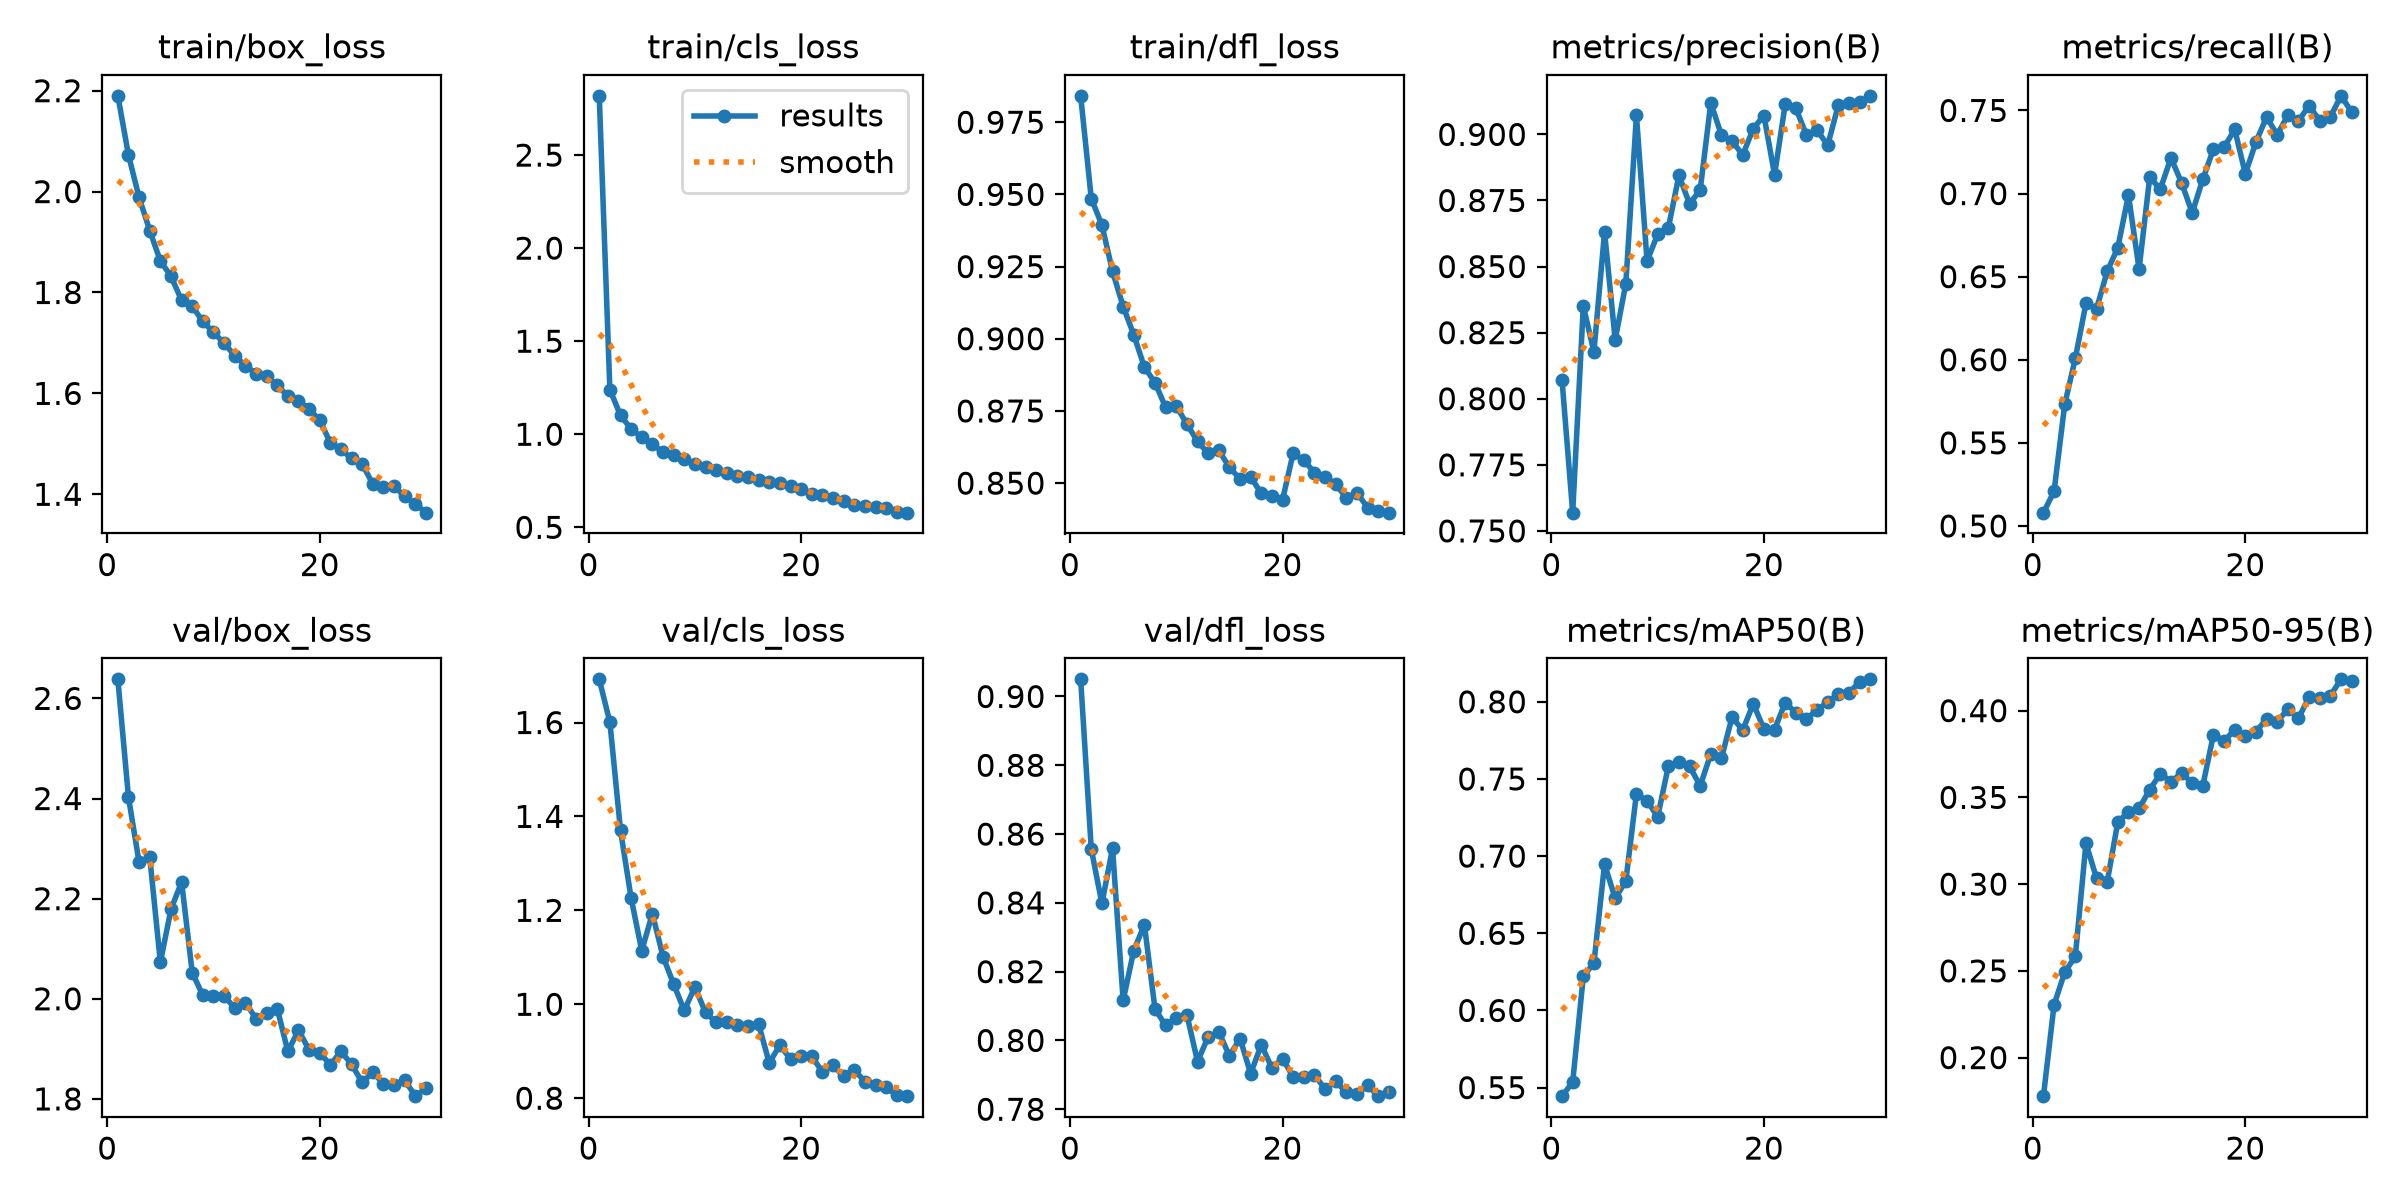
\includegraphics[width=0.47\textwidth]{images/pictures/training_curves_base.png}}
\hfill
\subfloat[YOLOv8n-P2-EMA]{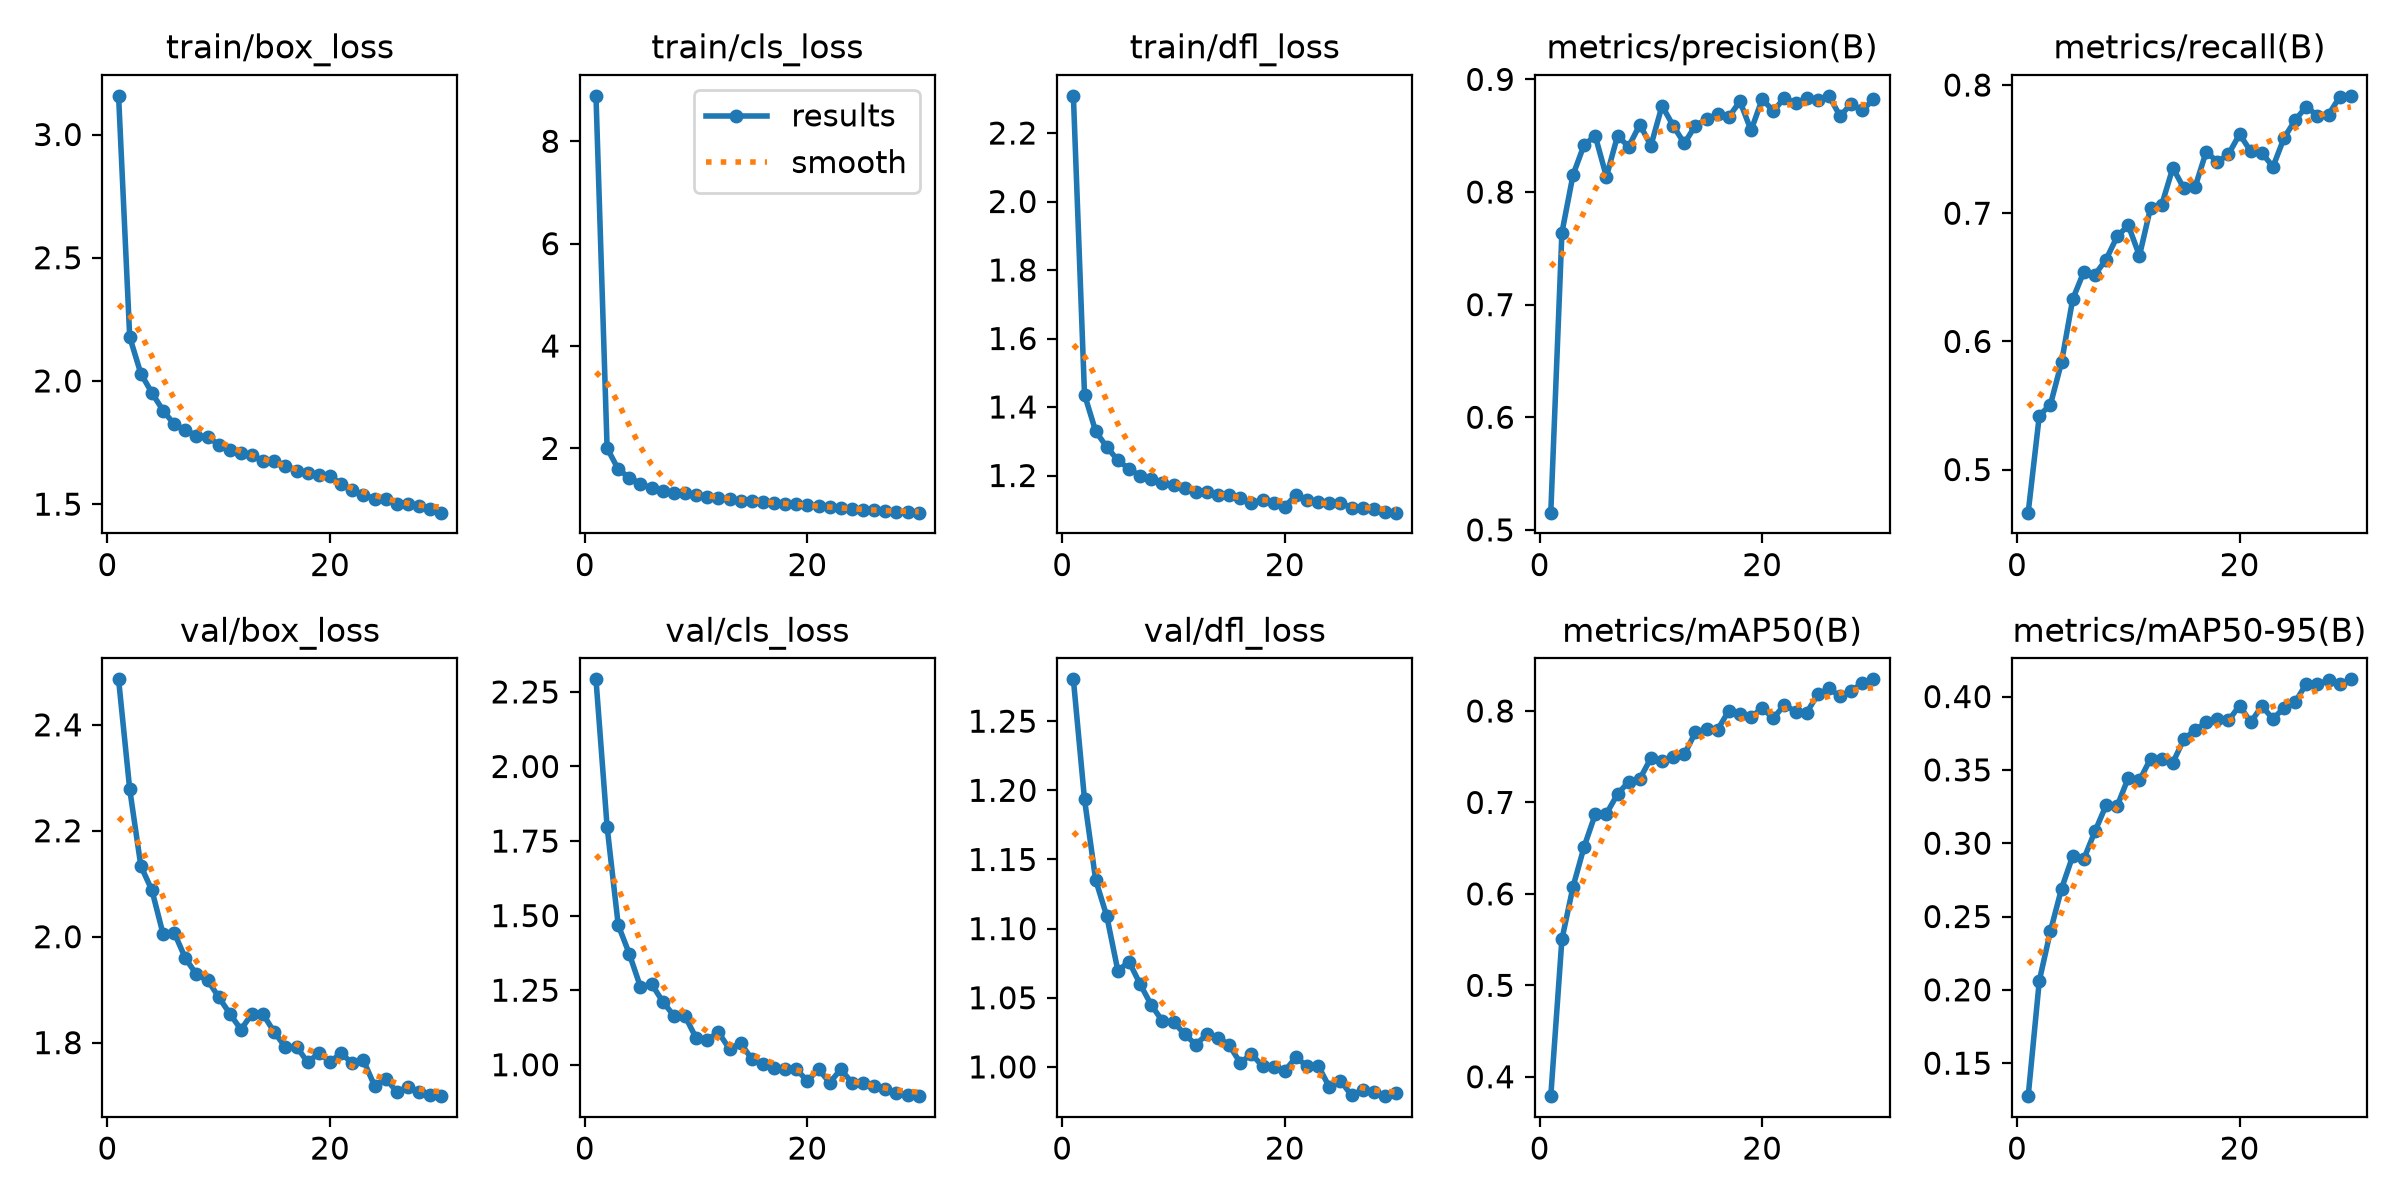
\includegraphics[width=0.47\textwidth]{images/pictures/training_curves_p2ema.png}}
\caption{训练损失与验证指标曲线}
\label{fig:training_curves}
\end{figure}

\section{消融实验}

\subsection{实验设置}

为验证 P2 与 EMA 各自的作用及组合效果，本文设计了四组对照实验：基线 YOLOv8n、+P2、+EMA、+P2+EMA。四组实验使用完全相同的数据划分、超参数与评测脚本，仅在网络结构上不同。评测在 Det-Fly 验证集上进行，输入 640，置信度阈值 0.001（mAP 计算需要低阈值以覆盖完整 P-R 曲线）。

\subsection{实验结果}

实验结果如表~\ref{tab:ablation} 所示。

\begin{table}[htbp]
\centering
\caption{检测模型消融实验（Det-Fly 验证集，imgsz=640）}
\label{tab:ablation}
\small
\begin{tabular}{lcccccccc}
\toprule
\textbf{模型} & \textbf{参数(M)} & \textbf{mAP50} & \textbf{mAP50-95} & \textbf{P} & \textbf{R} & \textbf{FPS} & \textbf{AP\_small} & \textbf{AP\_med} \\
\midrule
YOLOv8n（基线） & 3.01 & 81.3 & 41.8 & 91.2 & 75.9 & 123.0 & 6.1 & 77.0 \\
+P2 & 2.93 & 82.3 & 41.3 & 88.9 & 77.6 & 90.3 & 8.3 & 76.2 \\
+EMA & 3.02 & 76.2 & 36.3 & 85.5 & 72.2 & 101.0 & 4.1 & 75.0 \\
+P2+EMA（本文） & 2.94 & \textbf{83.5} & 41.2 & 88.2 & \textbf{79.2} & 98.4 & \textbf{9.8} & \textbf{78.0} \\
\bottomrule
\end{tabular}
\end{table}

表中所有指标单位为百分数，FPS 为帧每秒。AP\_small 为 COCO 面积口径、IoU=0.5、101 点插值。

\subsection{结果分析}

\textbf{（1）P2 单独作用}。mAP50 从 81.3\% 提升至 82.3\%，Recall 从 75.9\% 提升至 77.6\%，AP\_small 从 6.1\% 提升至 8.3\%，相对提升 36.1\%。这说明高分辨率检测层确实增强了小目标召回。与此同时，Precision 从 91.2\% 降至 88.9\%，mAP50-95 略降 0.5 个百分点，原因是 P2 层引入了更多弱响应，部分背景被误检。FPS 从 123 降至 90，符合计算量分析。

\textbf{（2）EMA 单独作用}。结果看似异常：mAP50 降至 76.2\%，AP\_small 仅 4.1\%，甚至低于基线。这一现象不能简单解释为"EMA 无效"。本文的分析是：EMA 的注意力重加权在缺乏高分辨率特征时，会把权重集中在 P3/P4 上已经模糊的目标区域，而这些区域的边界信息不足以支撑精确定位；同时，注意力对背景的抑制过于激进，导致部分低置信度的真实目标被"压"到阈值以下。换言之，EMA 需要一张"看得清"的特征图才能发挥"认得准"的作用。

\textbf{（3）P2+EMA 的互补性}。两者联合后，mAP50 达到 83.5\%，Recall 79.2\%，AP\_small 9.8\%，均为四组最优。AP\_small 相对基线提升 60.7\%，相对 +P2 提升 18.1\%。这一结果支持了"P2 提供分辨率、EMA 提供判别力"的解释：P2 让目标在特征图上占据足够多的网格，EMA 在这些网格上进一步区分目标与背景，二者形成正向互补。

\textbf{（4）参数效率}。本文模型的参数量为 2.94\,M，低于基线的 3.01\,M，却取得了最优的 mAP50 与 AP\_small。这说明性能提升并非来自模型容量扩张，而是来自特征利用效率的改善。对于部署在边缘设备上的反无人机系统，这一特性尤为重要。

\textbf{（5）速度}。本文模型 FPS 为 98.4，约为基线的 80\%，但仍为 30\,fps 视频帧率的 3 倍以上。考虑到系统还需要进行卡尔曼滤波、界面绘制与网络通信，保留 2--3 倍余量是必要的。

\subsection{混淆矩阵与 P-R 曲线}

图~\ref{fig:confusion} 给出了基线模型与本文模型的混淆矩阵。两者在"背景误检"上的差异不大，本文模型的漏检（真值为正、预测为背景）明显减少，这与 Recall 的提升一致。

\begin{figure}[htbp]
\centering
\subfloat[基线 YOLOv8n]{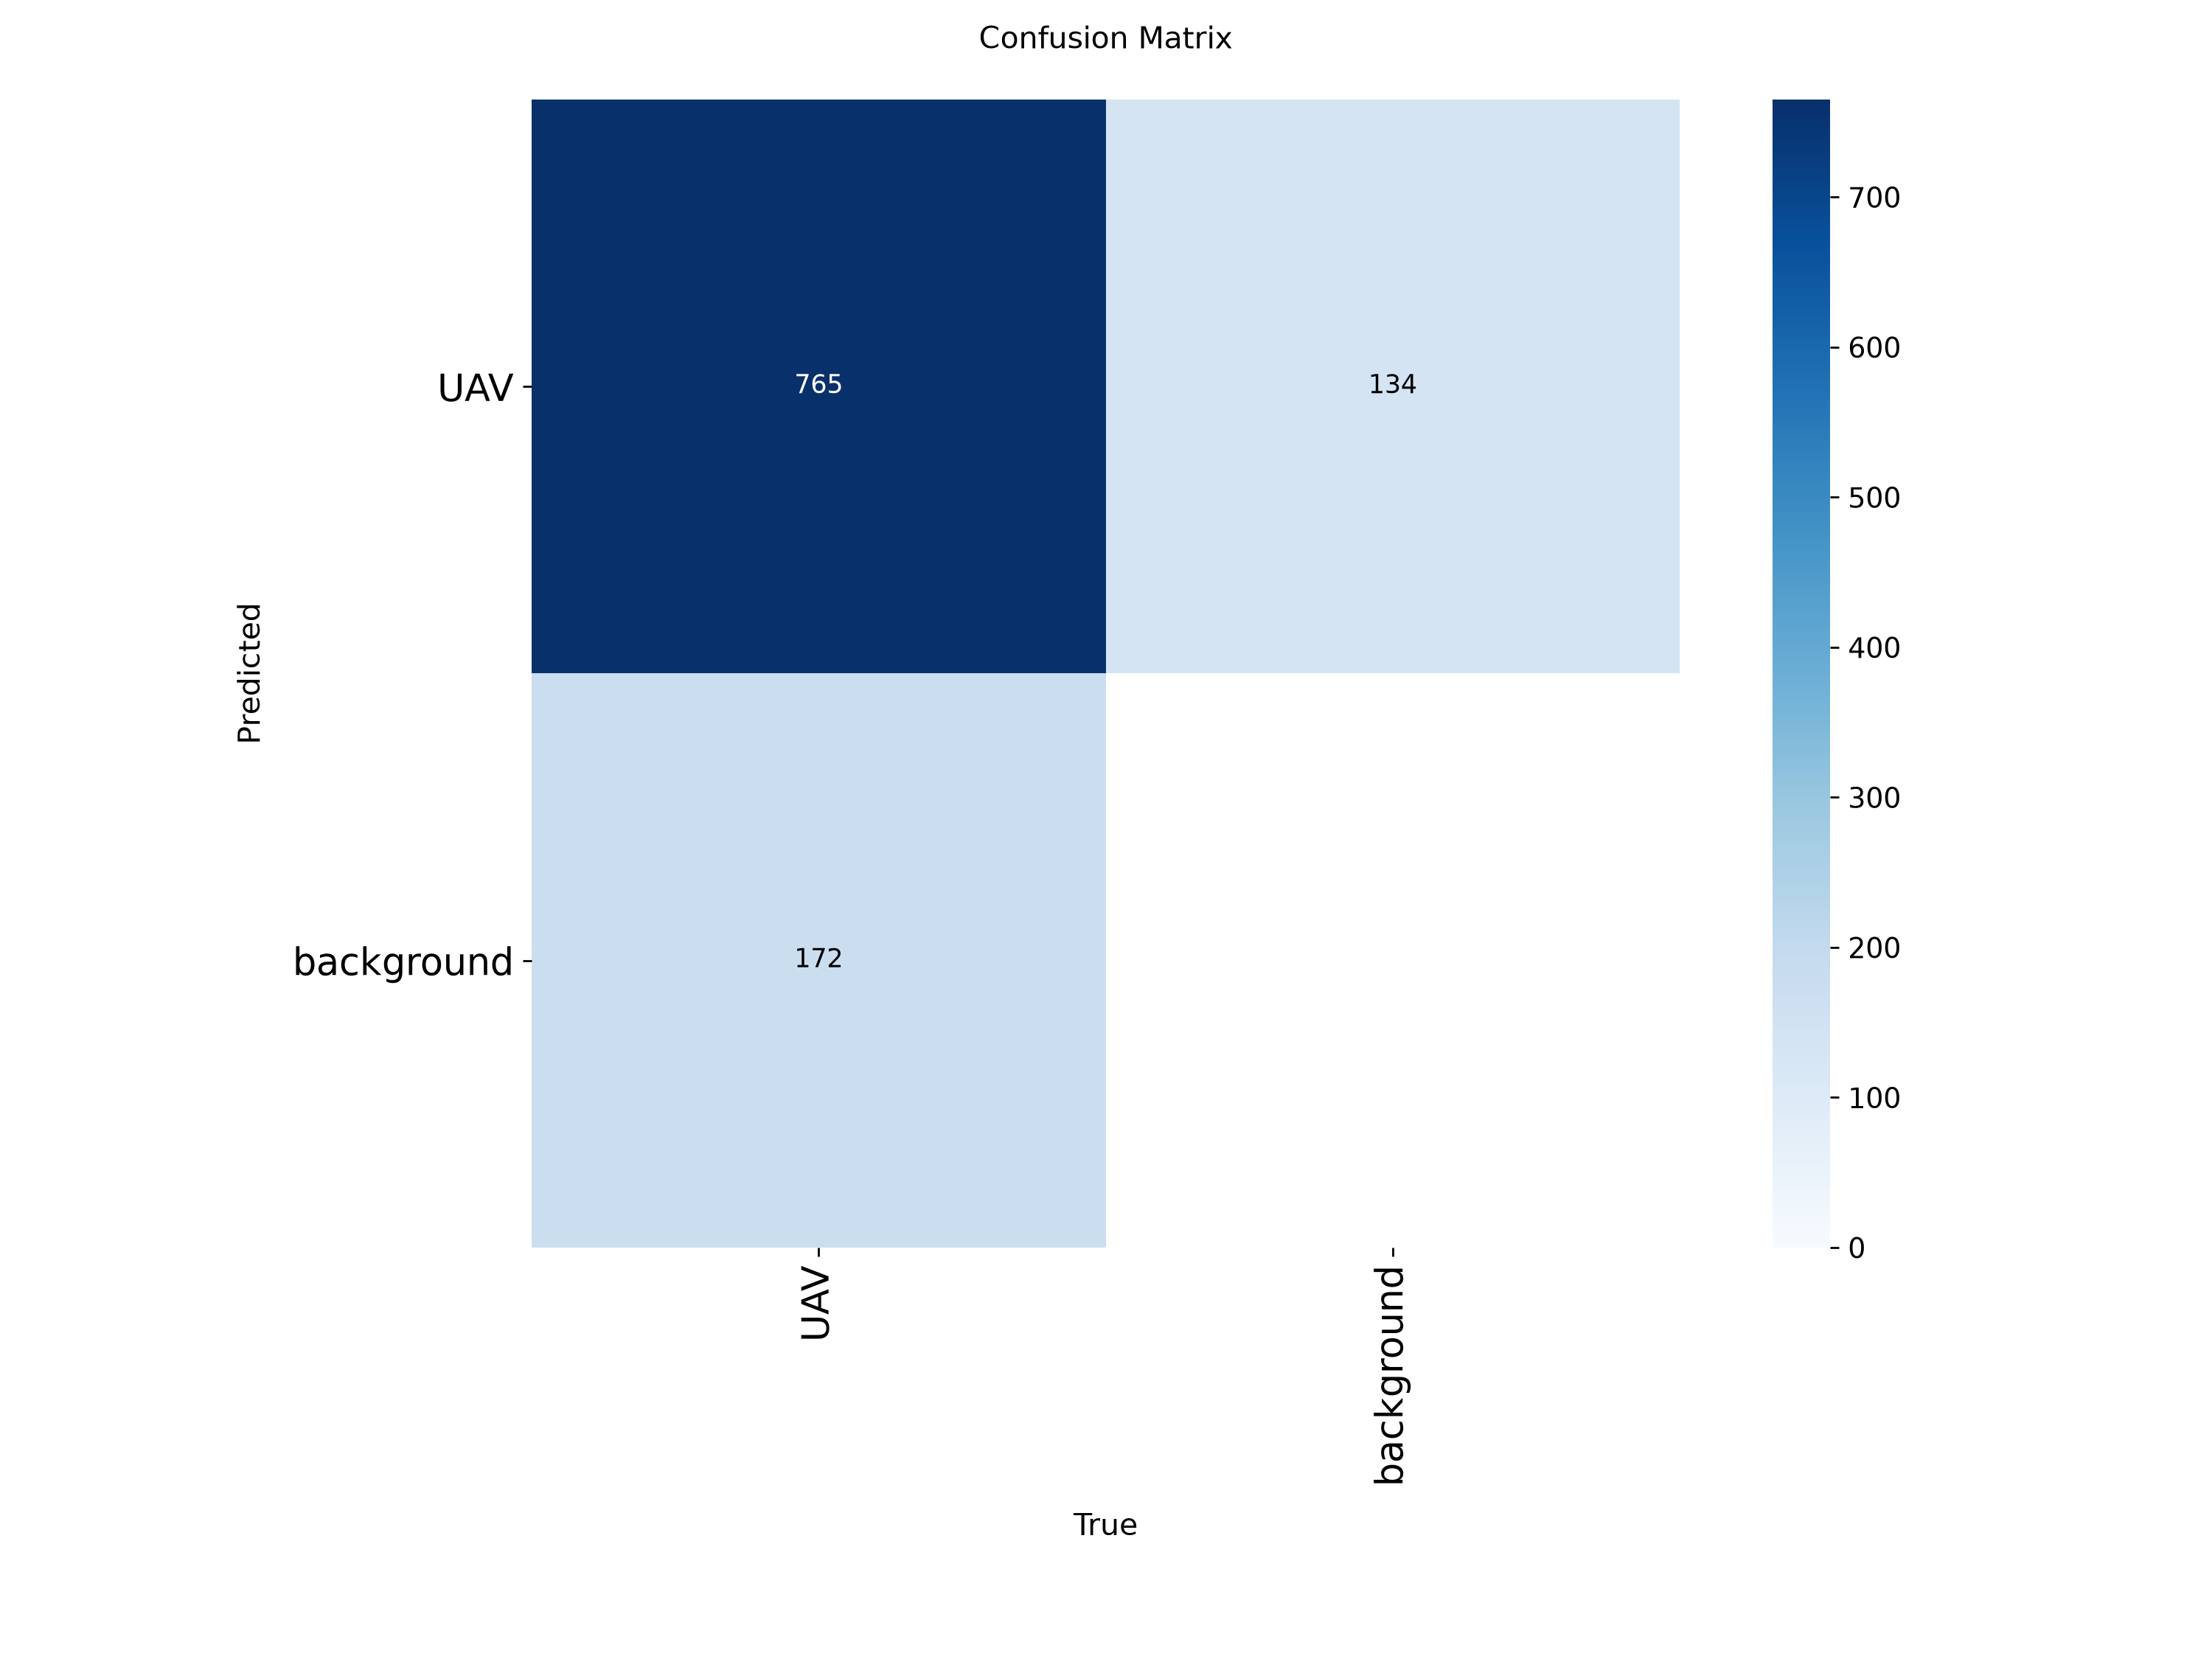
\includegraphics[width=0.45\textwidth]{images/pictures/confusion_matrix_base.png}}
\hfill
\subfloat[YOLOv8n-P2-EMA]{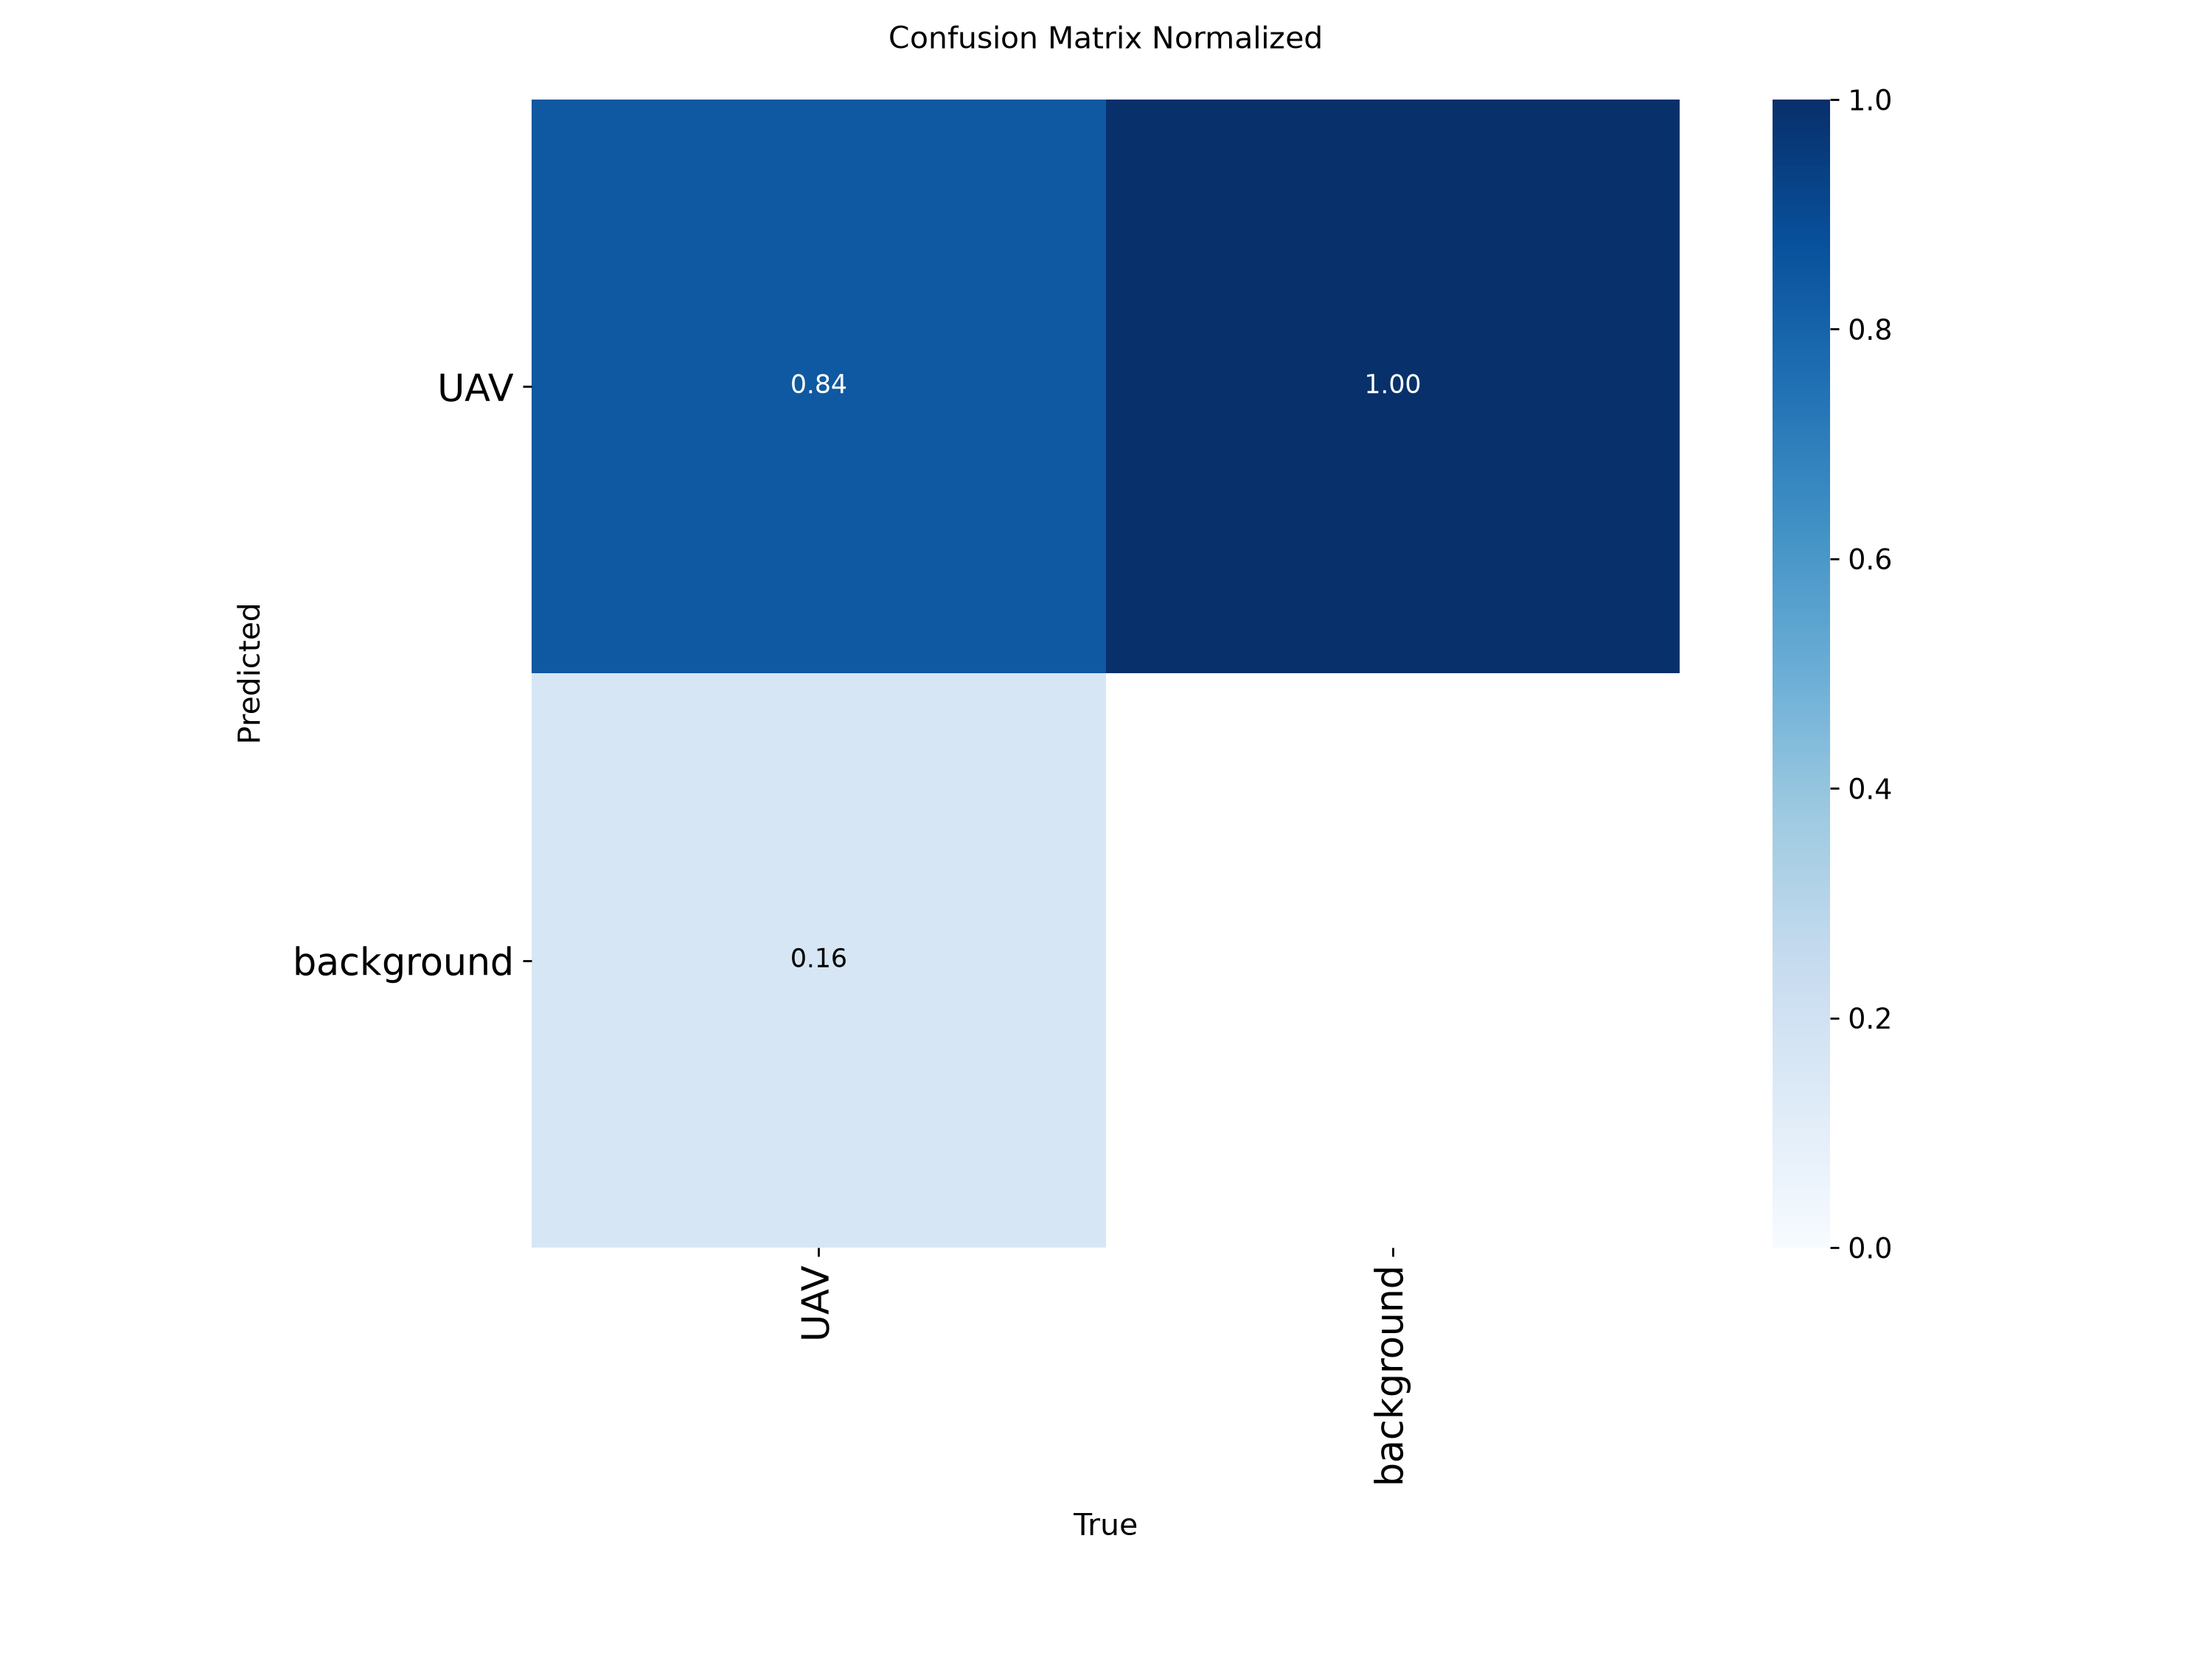
\includegraphics[width=0.45\textwidth]{images/pictures/confusion_matrix_p2ema.png}}
\caption{验证集混淆矩阵}
\label{fig:confusion}
\end{figure}

图~\ref{fig:pr_f1} 给出了本文模型的 P-R 曲线与 F1 曲线。P-R 曲线在高召回区间的"尾部"比基线更饱满，说明模型在低置信度区域仍能保持一定的精度，这对后续状态机的低门限初筛是有利的。

\begin{figure}[htbp]
\centering
\subfloat[P-R 曲线]{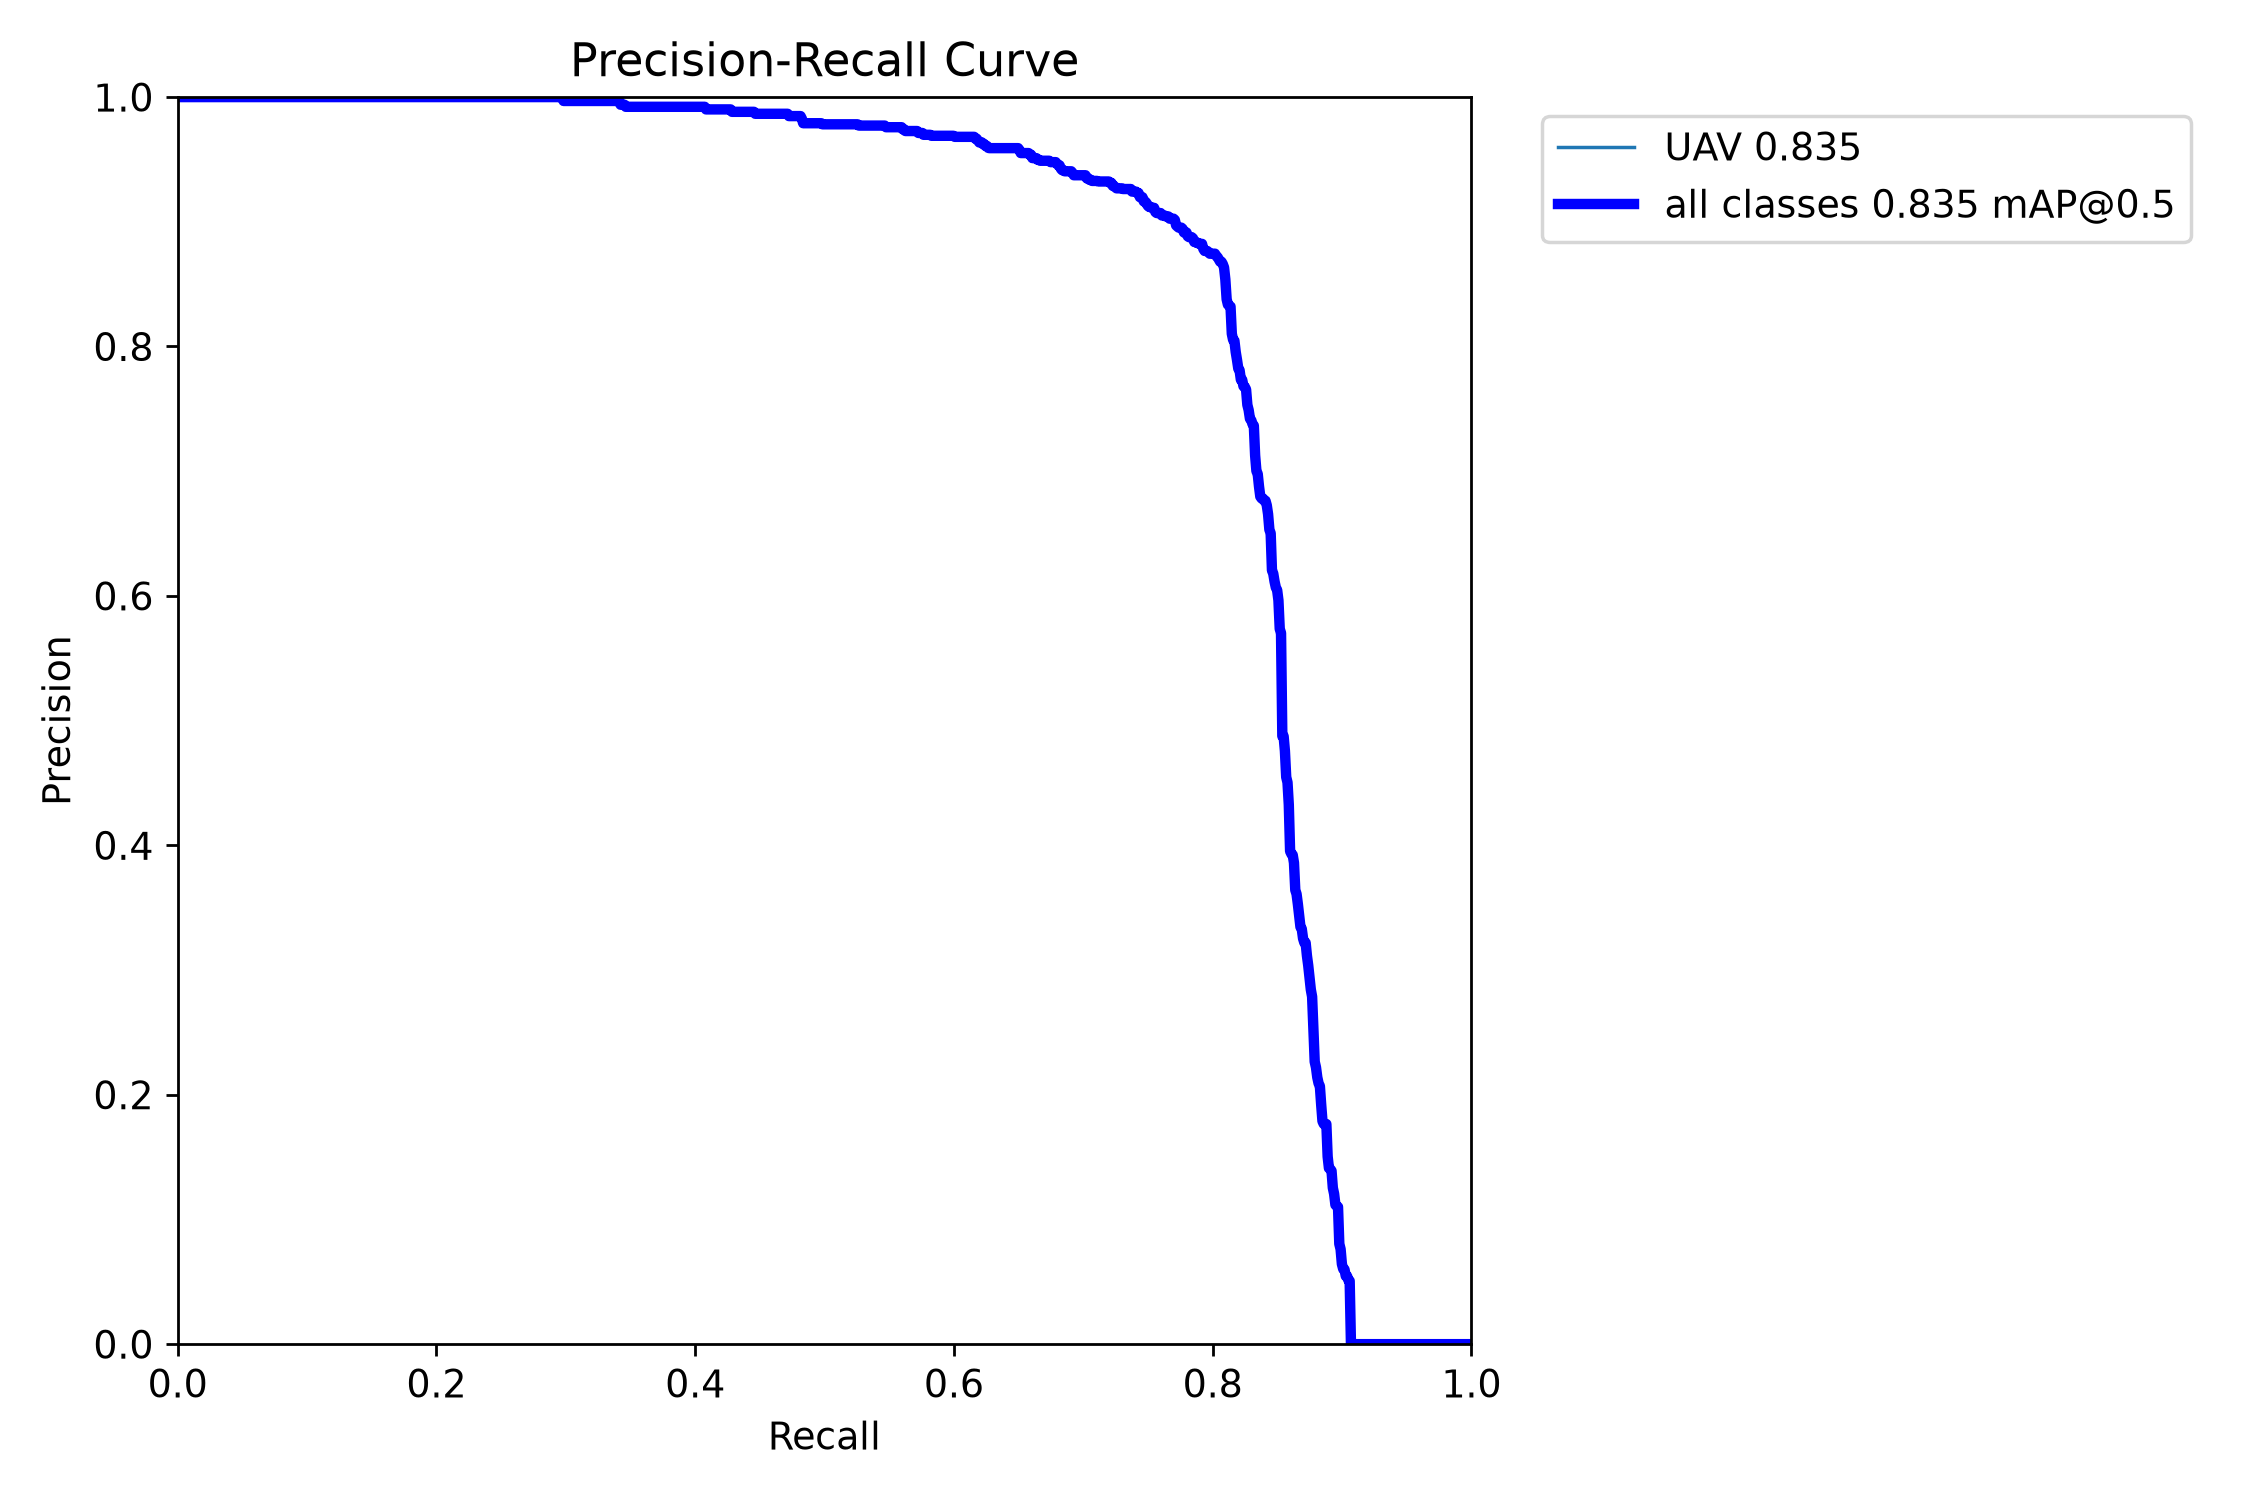
\includegraphics[width=0.47\textwidth]{images/pictures/pr_curve_p2ema.png}}
\hfill
\subfloat[F1-置信度曲线]{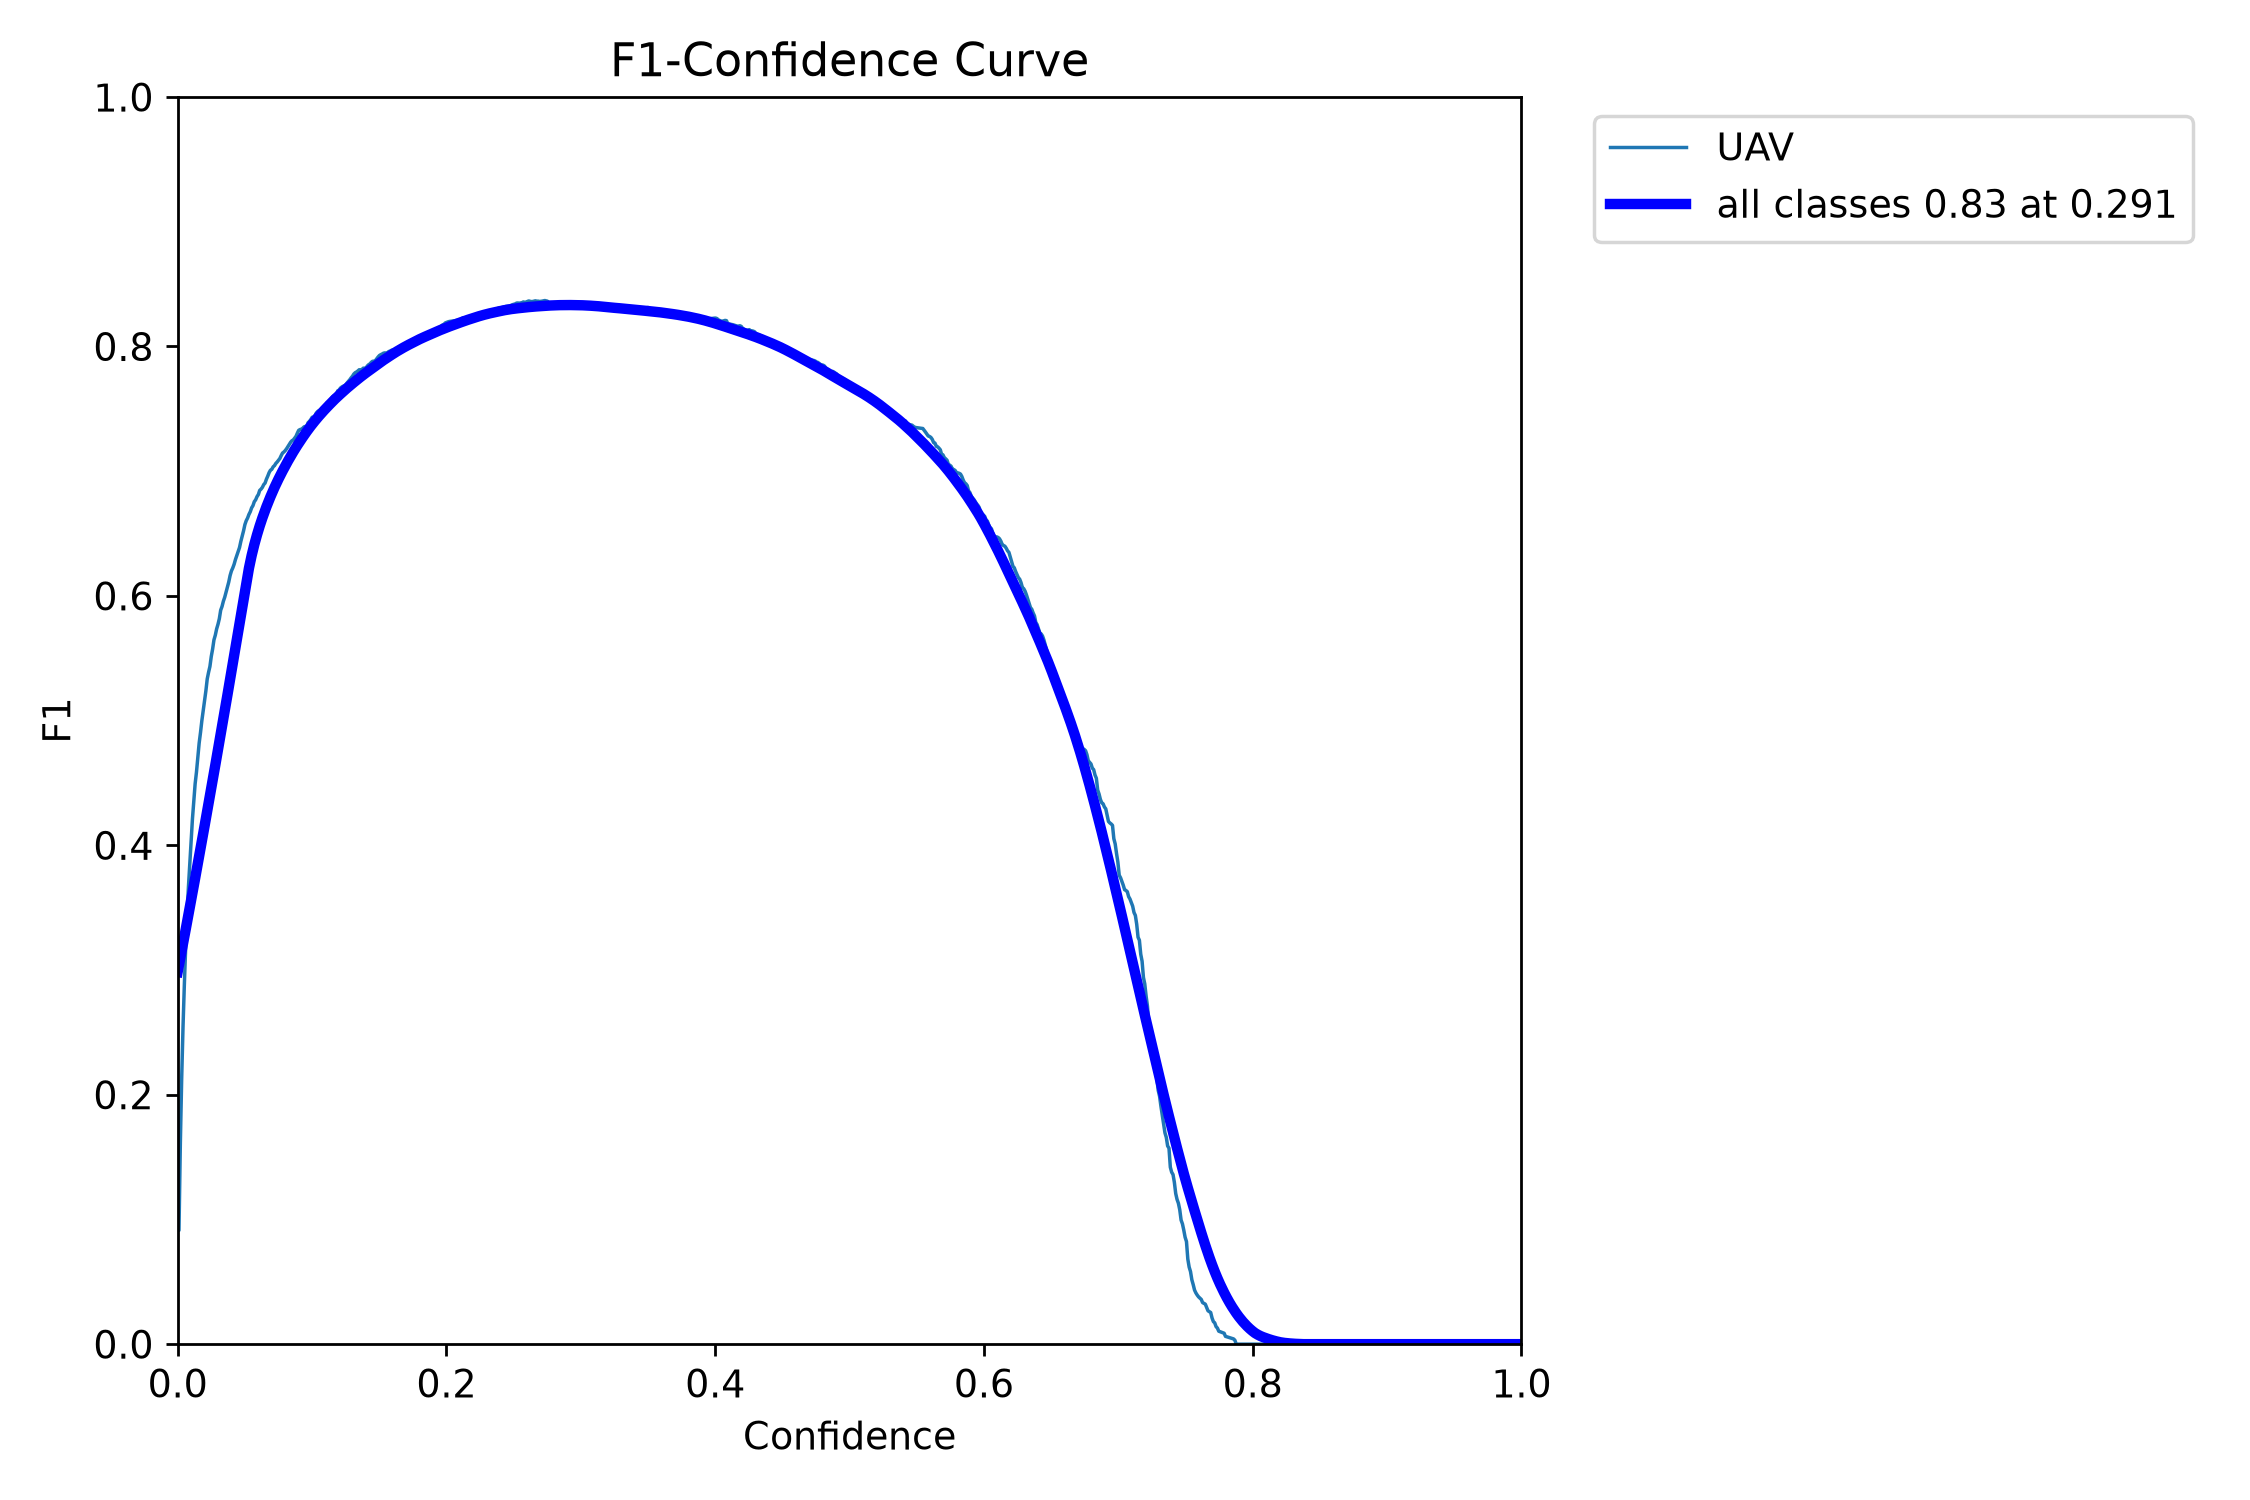
\includegraphics[width=0.47\textwidth]{images/pictures/f1_curve_p2ema.png}}
\caption{YOLOv8n-P2-EMA 的 P-R 与 F1 曲线}
\label{fig:pr_f1}
\end{figure}

\subsection{检测效果可视化}

图~\ref{fig:val_predictions} 展示了验证集的批量预测结果。绿色框为真值，红色框为预测。可以看到，本文模型在目标较小、背景复杂的场景中仍能给出稳定的框，框的边界与真值吻合较好。

\begin{figure}[htbp]
\centering
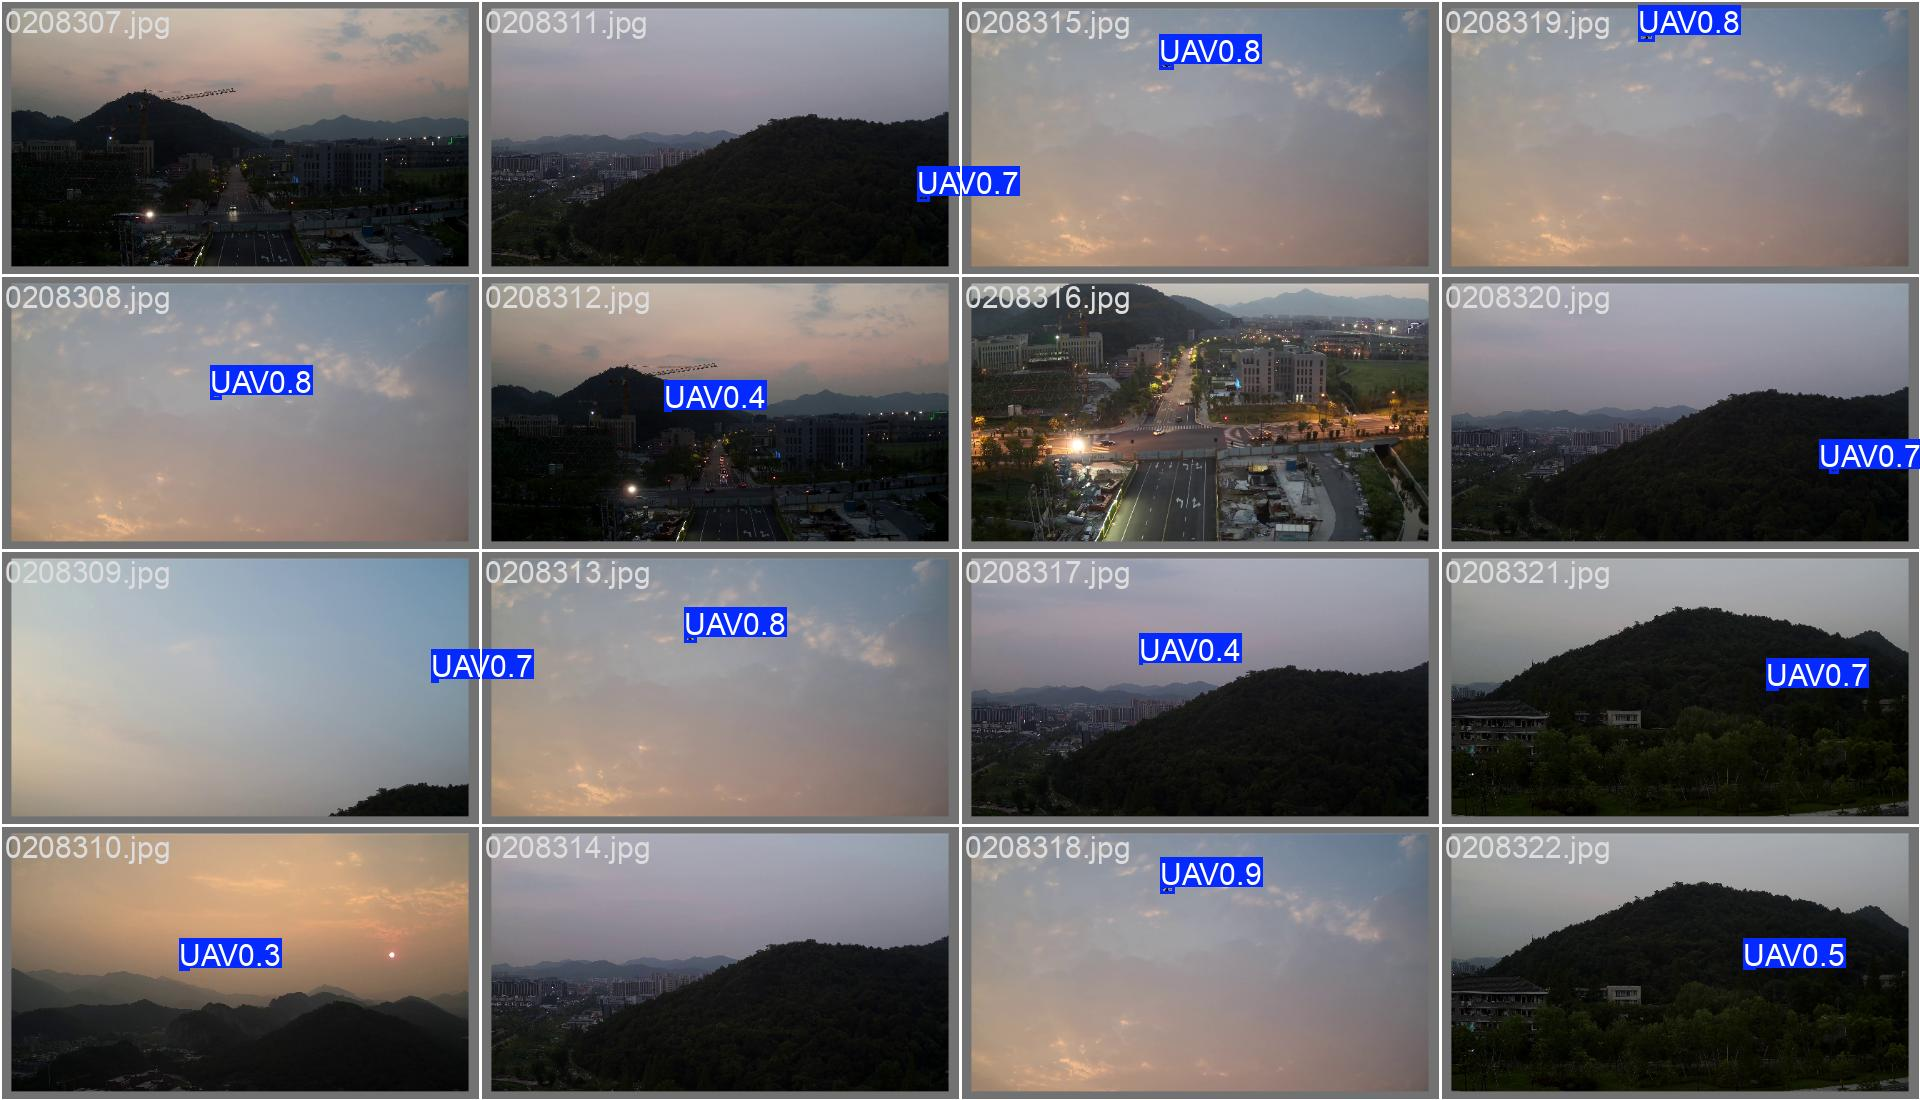
\includegraphics[width=0.92\textwidth]{images/pictures/val_predictions.jpg}
\caption{验证集批量预测结果（绿框为真值，红框为预测）}
\label{fig:val_predictions}
\end{figure}

图~\ref{fig:compare} 给出了四组典型帧的对比，按"基线置信度与本文置信度差异"排序选取，用于直观展示改进在困难样本上的效果。蓝色虚线框为真值，实线框为预测。

\begin{figure}[htbp]
\centering
\subfloat[样本一]{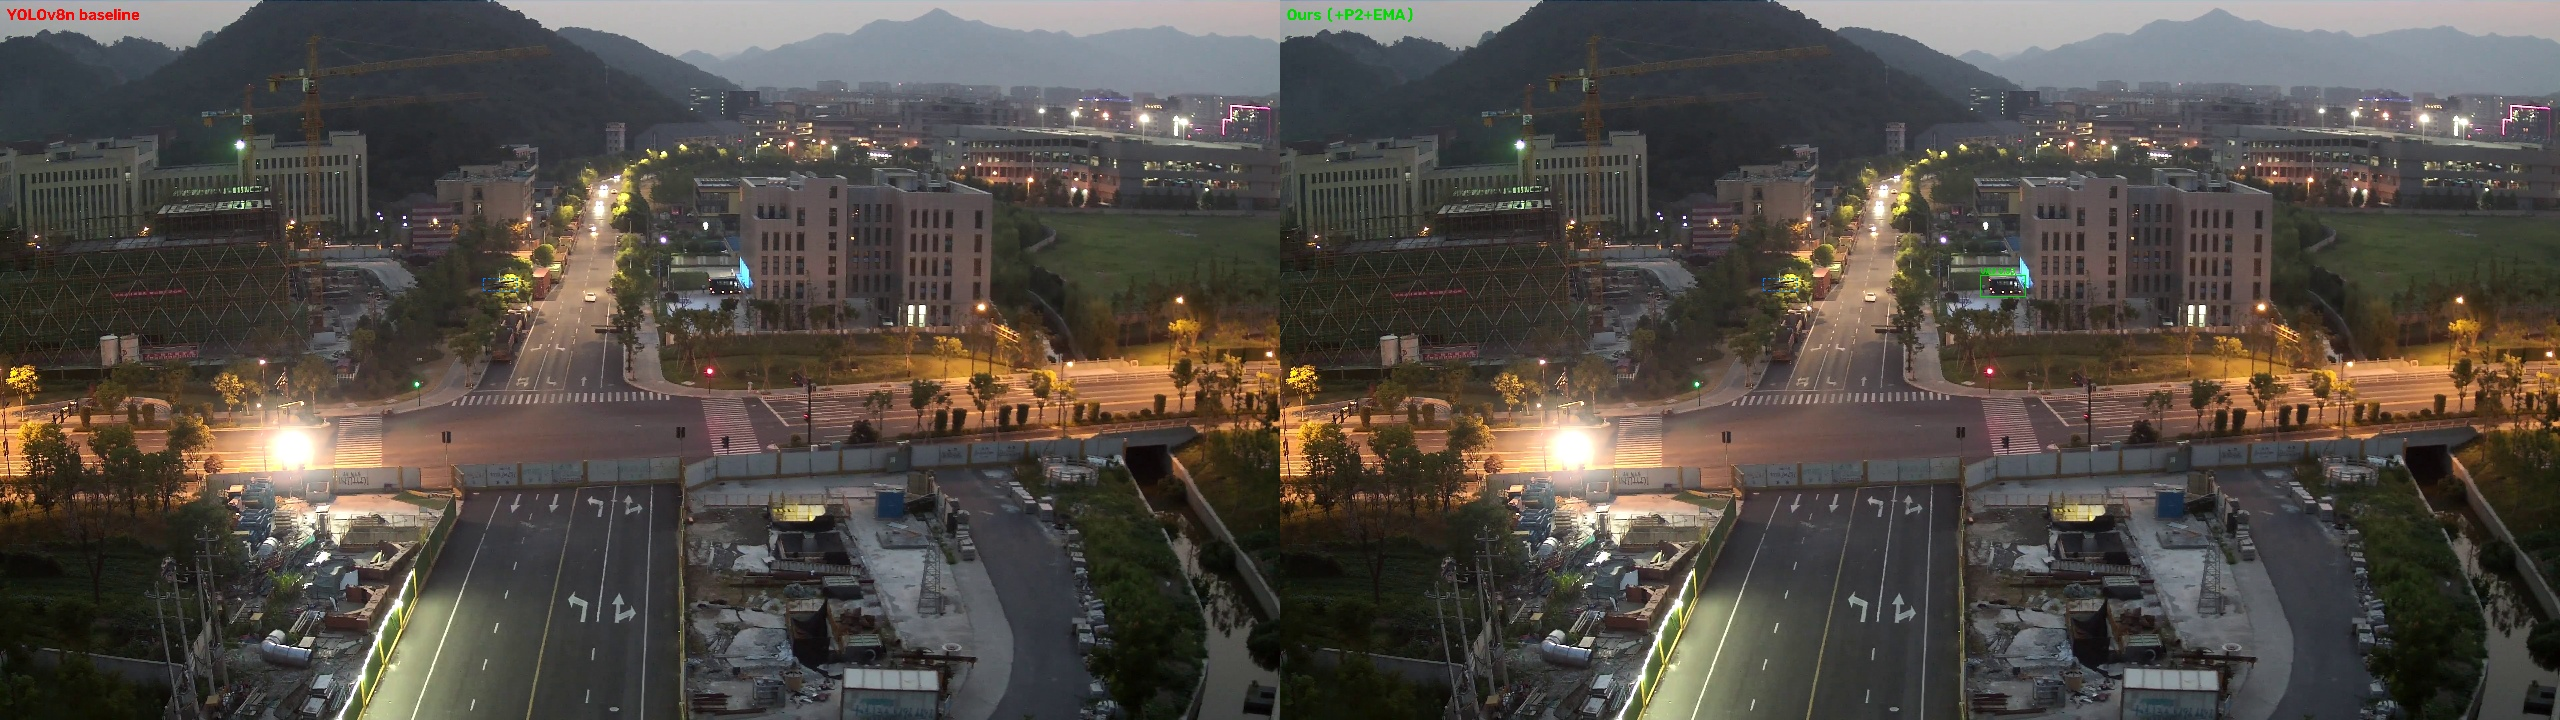
\includegraphics[width=0.48\textwidth]{images/pictures/compare_01.jpg}}
\hfill
\subfloat[样本二]{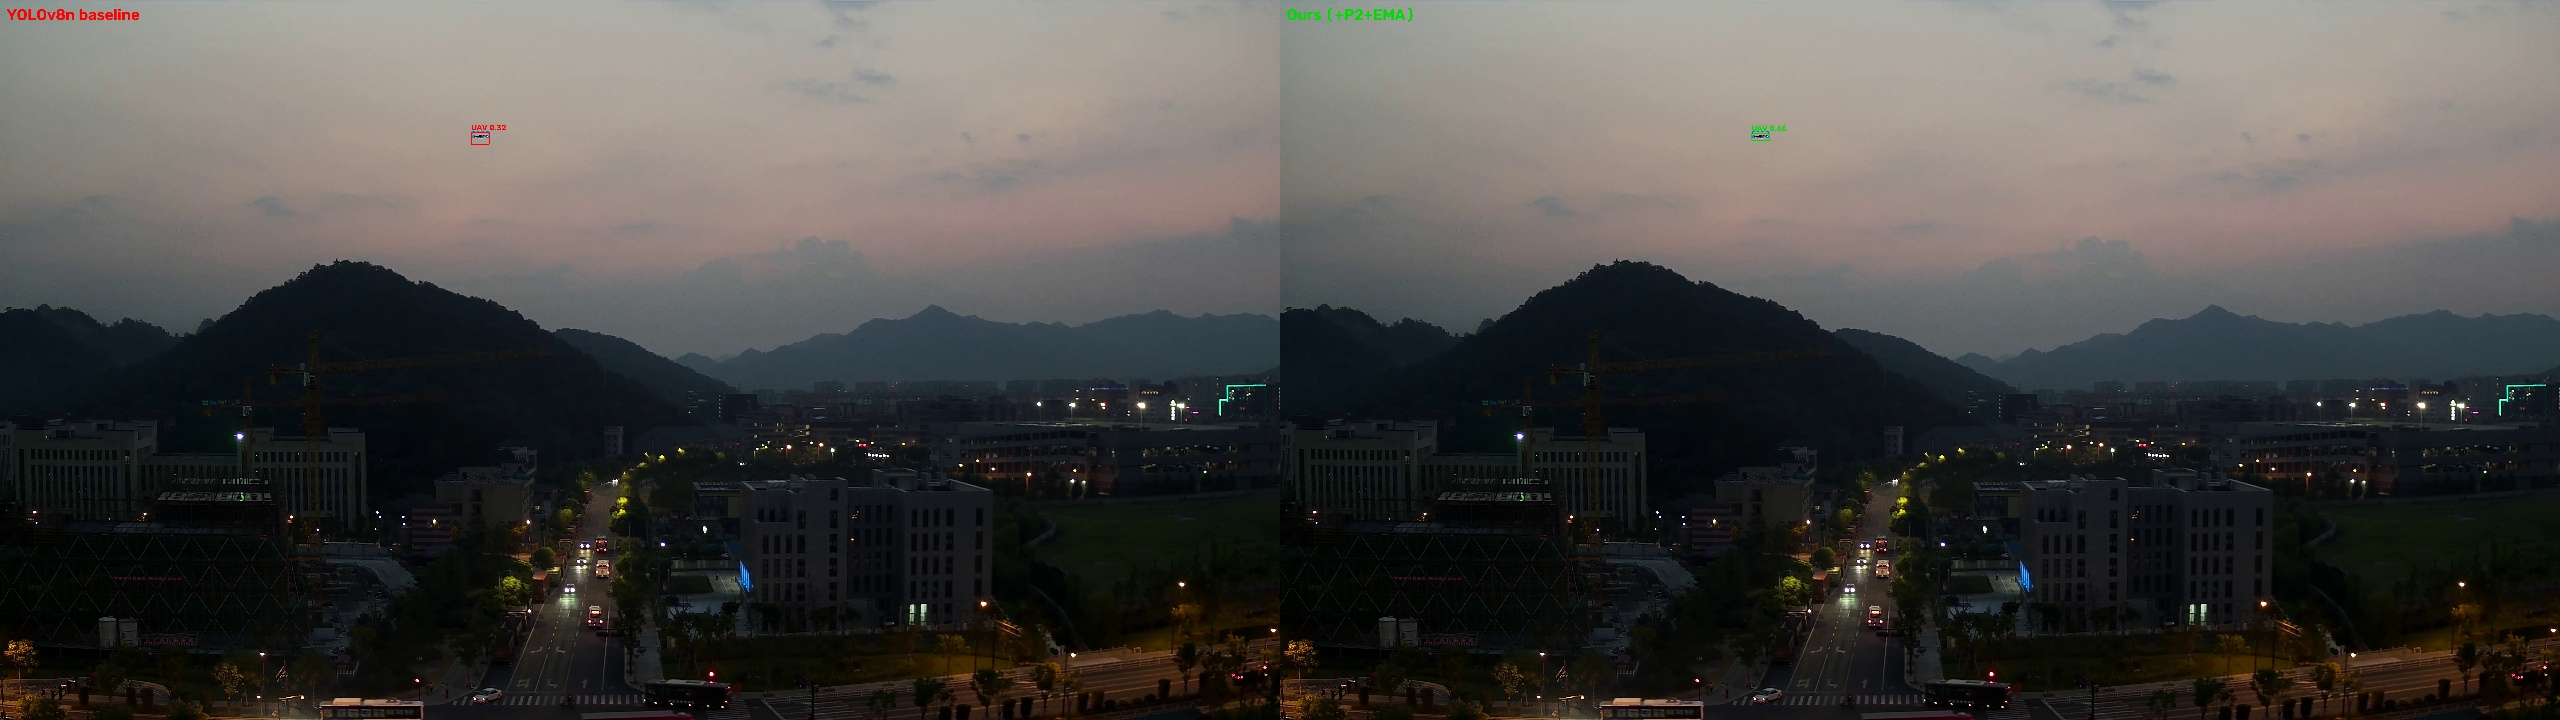
\includegraphics[width=0.48\textwidth]{images/pictures/compare_02.jpg}}\\
\subfloat[样本三]{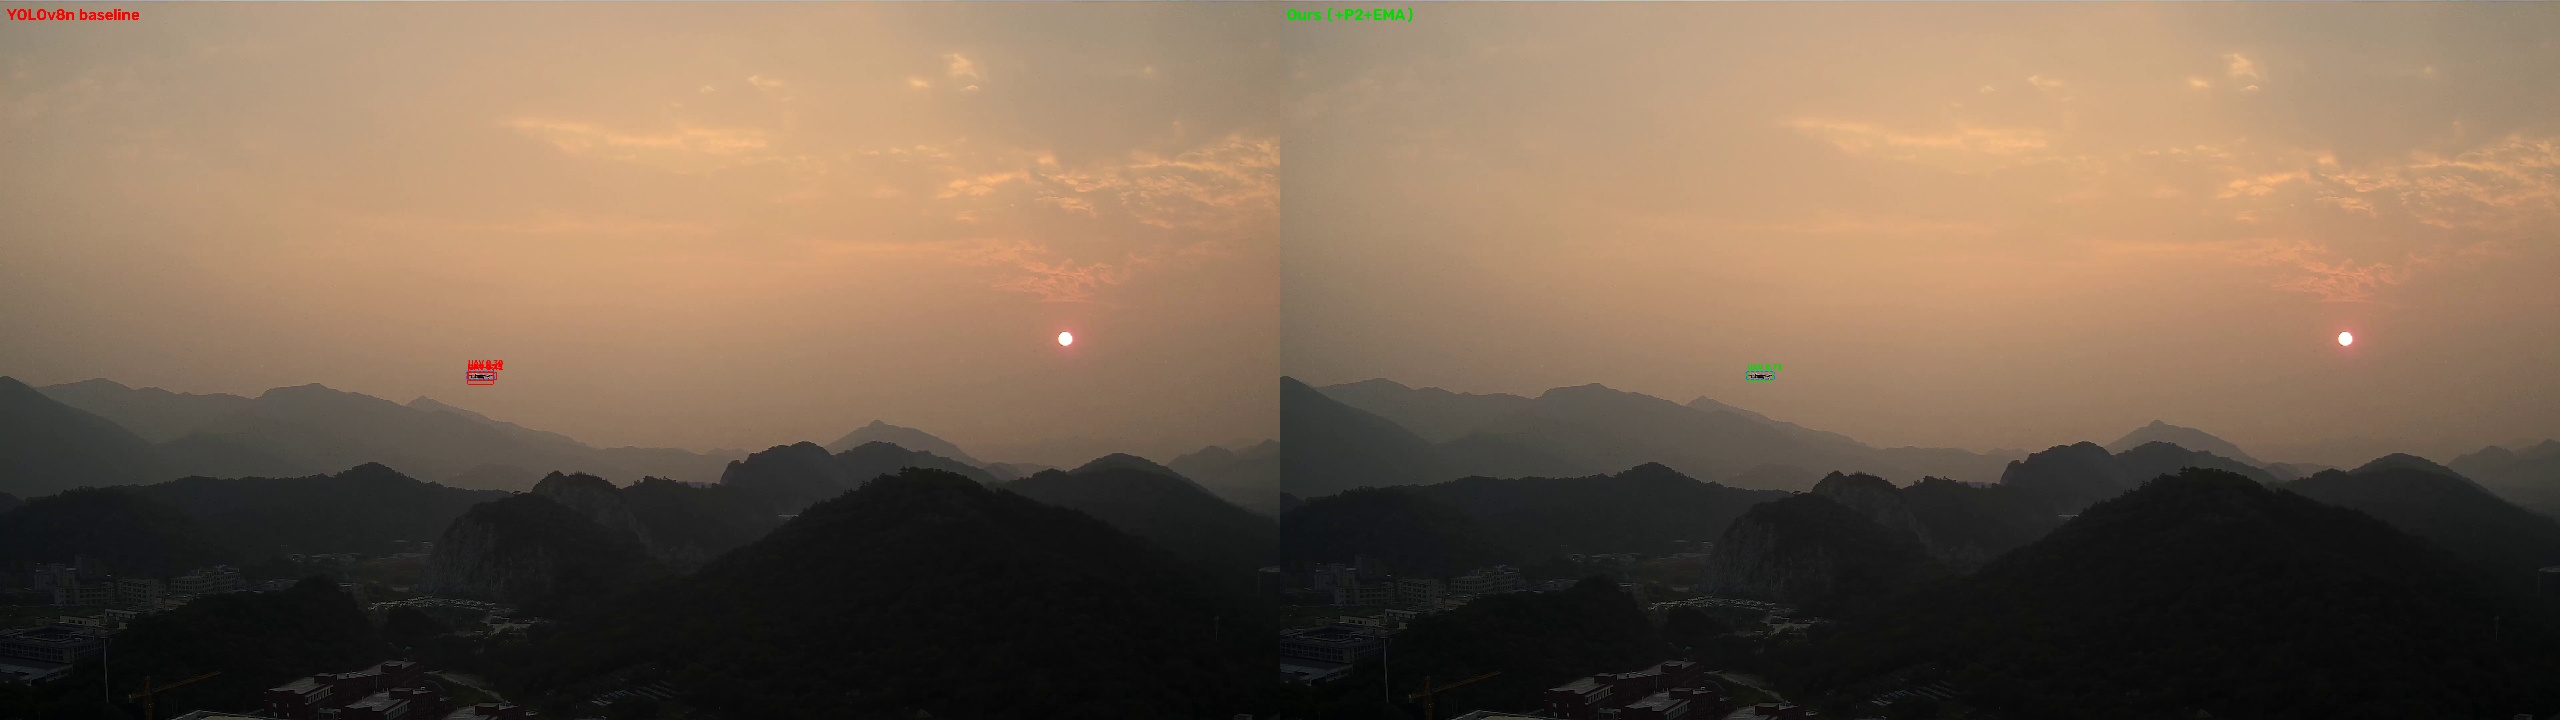
\includegraphics[width=0.48\textwidth]{images/pictures/compare_03.jpg}}
\hfill
\subfloat[样本四]{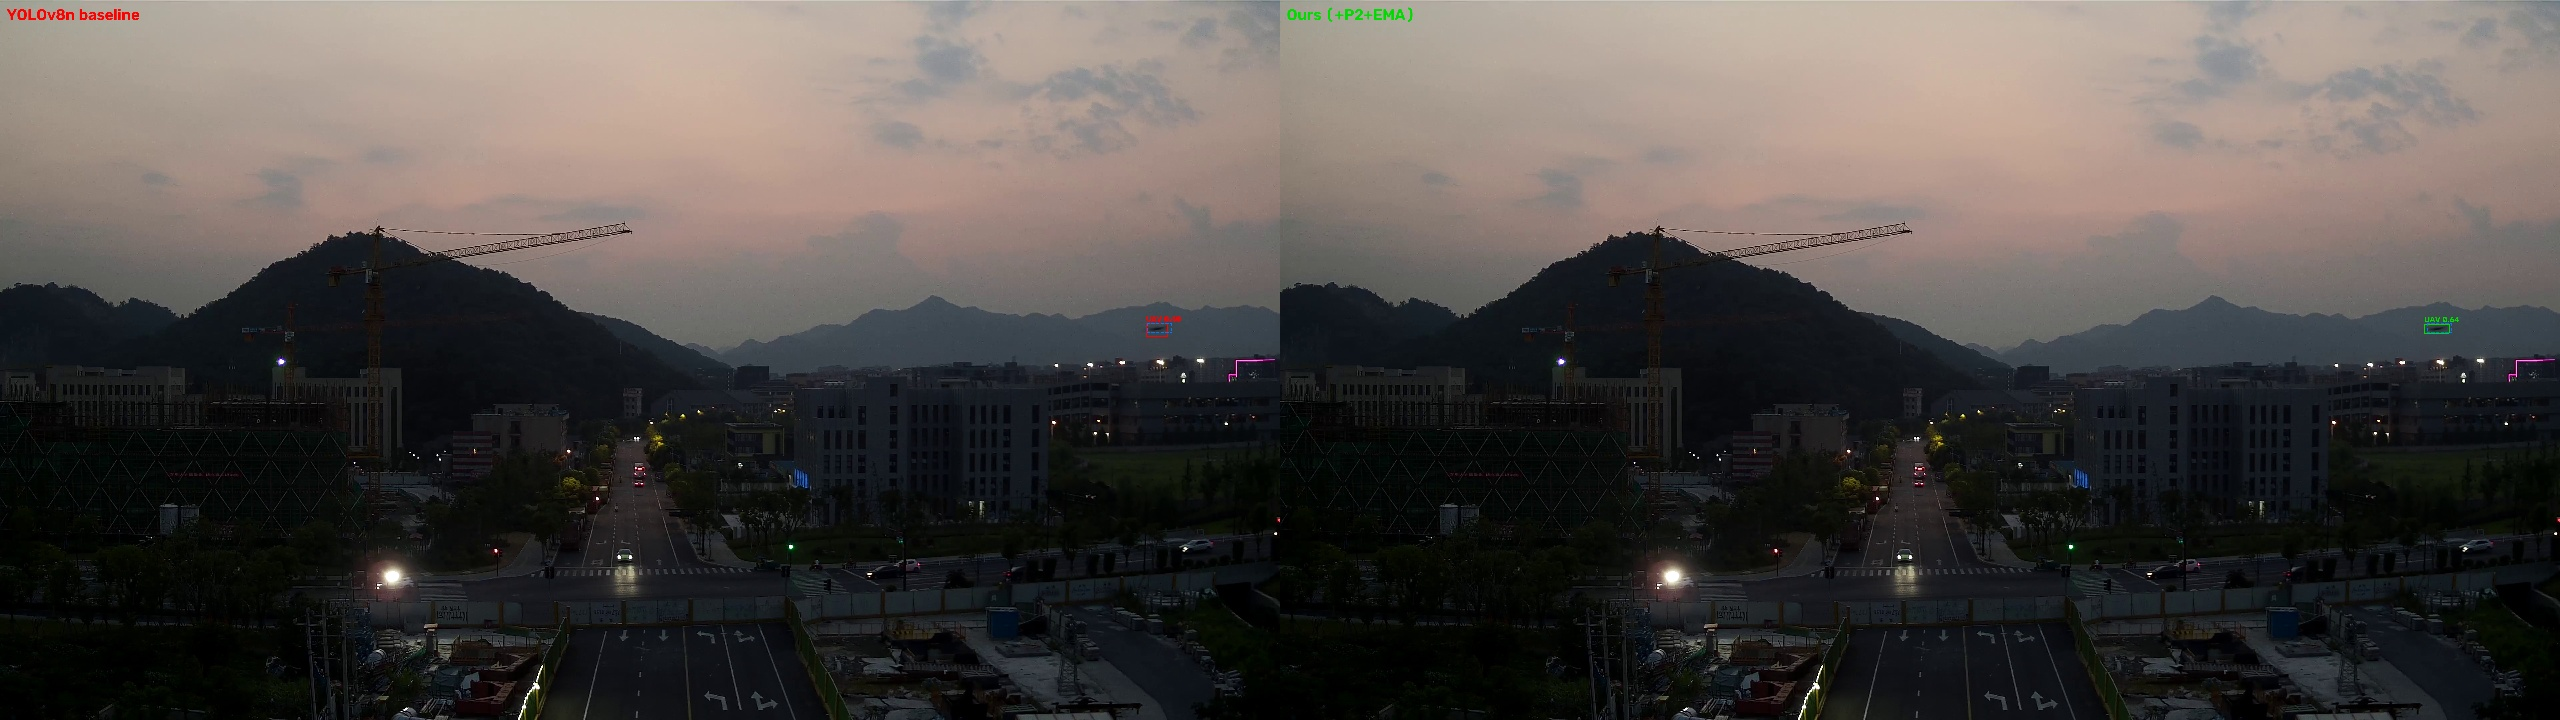
\includegraphics[width=0.48\textwidth]{images/pictures/compare_04.jpg}}
\caption{基线与本文模型的典型帧对比}
\label{fig:compare}
\end{figure}

\section{与非 YOLO 方法的横向讨论}

Det-Fly 数据集上已有 Faster R-CNN\cite{faster_rcnn}、SSD\cite{ssd} 与 RT-DETR\cite{rt_detr} 等方法的评测结果。需要说明的是，这些结果来自不同论文，数据划分、输入尺寸与训练轮次并不统一，直接比较数值并不严谨。本文仅做定性讨论。

两阶段方法 Faster R-CNN 的优势在于区域建议机制能够对候选区域做二次细化，对极小目标的定位精度较高；劣势是推理速度慢，难以满足实时监视需求。单阶段方法 SSD 速度较快，但其特征金字塔的浅层语义较弱，小目标召回有限。Transformer 方法 RT-DETR 通过集合预测避免了 NMS，在密集小目标场景中表现较好，但计算量与显存占用显著高于 YOLOv8n。

本文方法在保持 nano 级参数量的前提下，通过 P2 与 EMA 提升了小目标能力，其定位是"在边缘设备上可实时运行的小目标检测方案"，而非追求绝对精度最优。这一定位与反无人机系统的实际部署条件相符。

\section{有效工作范围与失效模式}

\subsection{置信度与目标尺度的关系}

检测模型的置信度随目标在画面中的尺度变化而显著变化。本文在仿真环境中做了系统测量（详见第七章），发现未微调模型在目标占画面高度约 1/5 以上时置信度接近 0，在目标过小时置信度低于 0.25。前者属于训练分布外的大尺度输入，后者属于信息不足。模型的有效工作窗口约为目标高度占画面的 1/20 至 1/8。

这一现象提示：检测模型的能力不能只用 mAP 概括，必须结合部署场景的尺度分布评估。对于反无人机系统，这意味着需要通过镜头焦距、安装高度与告警距离的综合设计，使目标在告警时落在有效窗口内。

\subsection{典型失效模式}

本文观察到三类典型失效。

（1）\textbf{背景纹理误检}。树叶缝隙、建筑窗户的反光、天空中的云边缘在低分辨率下与无人机轮廓相似，模型可能给出 0.2--0.4 的置信度。这类误检通常置信度不高，可被初锁门限过滤，但在 SEARCH 状态下会造成短暂的候选框闪烁。

（2）\textbf{多目标粘连}。当画面中出现两架以上无人机且距离较近时，检测框可能合并，导致后续跟踪时目标身份不清。本文的系统面向单目标场景，未专门处理该情况。

（3）\textbf{极端光照}。逆光、夜间与强反光条件下，目标轮廓与背景的对比度下降，检出率显著降低。第四章的退化实验表明，P2+EMA 在暗光条件下相对基线有明显优势，但仍无法与正常光照相比。

\section{本章小结}

本章以 YOLOv8n 为基础，引入 P2 高分辨率检测头与 EMA 注意力，构建了面向无人机小目标的检测模型。消融实验表明：P2 单独使用可提升召回与 AP\_small，但会引入少量误检；EMA 单独使用会因缺乏高分辨率特征而性能下降；二者联合后取得最优的 mAP50 83.5\%、Recall 79.2\% 与 AP\_small 9.8\%，且参数量低于基线。本章从特征分辨率与注意力重加权两个角度解释了这一互补关系，并讨论了模型的有效工作范围与三类典型失效模式，为后续章节的状态机设计与仿真域微调提供了依据。
